% !TeX program = lualatex
% !TeX root = main.tex
\documentclass[12pt,a4paper,oneside,openany]{report}
% ---------------------------------------------------------
% TESI TRIENNALE - TOR VERGATA
% Modifica il frontespizio e l'impaginazione in questo file.
% ---------------------------------------------------------
\usepackage[italian]{babel}
\usepackage{fontspec}
\setmainfont{Latin Modern Roman}
\setsansfont{Latin Modern Sans}
% Font monospaziato discreto per gli identificatori nel testo.
\setmonofont{Latin Modern Mono}[Scale=0.95]
% Nei listati manteniamo il font DejaVu, leggibile e compatibile con l'albero AST.
\newfontfamily\codeblockfont{DejaVu Sans Mono}[Scale=0.95]
\usepackage{amsmath,amssymb,mathtools}
\usepackage[a4paper,top=2.8cm,bottom=2.8cm,left=3.15cm,right=2.65cm,headheight=16pt]{geometry}
\usepackage{microtype}
\usepackage{newunicodechar}
\usepackage{multirow}
% Unicode symbols present in the supplied Markdown text.
\newunicodechar{ε}{\ensuremath{\varepsilon}}
\newunicodechar{↳}{\ensuremath{\hookrightarrow}}
\usepackage{graphicx}
\usepackage{float}
\usepackage{placeins}
\usepackage{longtable,booktabs,array,calc}
\usepackage{etoolbox}
\AtBeginEnvironment{longtable}{\footnotesize}
\usepackage{fancyvrb}
\usepackage{fvextra}
\usepackage[table]{xcolor}
\usepackage{enumitem}
\usepackage{csquotes}
\usepackage{xurl}
\usepackage{hyperref}
\usepackage{bookmark}
\usepackage[backend=biber,style=numeric,sorting=none,giveninits=true,doi=true,url=true,isbn=false]{biblatex}
\usepackage{tabularx}
\usepackage{listings}
\usepackage{caption}
\usepackage{needspace}

\lstdefinestyle{tesicode}{
    basicstyle=\codeblockfont\fontsize{9.3}{11.1}\selectfont,
    backgroundcolor=\color{blue!3},
    frame=single,
    rulecolor=\color{blue!25!gray},
    framesep=4pt,
    xleftmargin=4pt,
    xrightmargin=4pt,
    breaklines=true,
    breakatwhitespace=false,
    columns=fullflexible,
    keepspaces=true,
    showstringspaces=false,
    upquote=true,
    aboveskip=6pt,
    belowskip=6pt,
    postbreak={},
    prebreak={},
}

\lstset{style=tesicode}

\captionsetup[table]{
    font=small,
    labelfont=normalfont,
    justification=centering,
    singlelinecheck=true,
    skip=5pt
}

\addbibresource{bibliografia_tesi.bib}
\definecolor{tesiblu}{RGB}{34,75,117}
\hypersetup{colorlinks=true,linkcolor=tesiblu,citecolor=tesiblu,urlcolor=tesiblu,
  pdftitle={A Domain-Specific Language for Security Assurance of 5G SCAS Tests from Network Traffic Captures},
  pdfauthor={Samuele De Santis}}
\graphicspath{{figure/}}
% Stile dei listati DSL, Python, Lark e MFOTL
\RecustomVerbatimEnvironment{verbatim}{Verbatim}{
    formatcom=\codeblockfont,
    fontsize=\small,
    breaklines=true,
    breakanywhere=true,
    tabsize=4,
    frame=single,
    framerule=0.4pt,
    framesep=7pt,
    rulecolor=\color{blue!25!gray},
    fillcolor=\color{blue!3},
    xleftmargin=4pt,
    xrightmargin=4pt,
    breaksymbolleft={},
    breaksymbolright={}
}
\setlength{\parindent}{1.05em}
\setlength{\parskip}{0.25em}
\setlist{nosep,topsep=0.3em}
\renewcommand{\arraystretch}{1.15}
\emergencystretch=2em
\clubpenalty=10000
\widowpenalty=10000
\displaywidowpenalty=10000
\sloppy
% Pandoc helpers:
\providecommand{\tightlist}{\setlength{\itemsep}{0pt}\setlength{\parskip}{0pt}}
\providecommand{\real}[1]{#1}
% References, tables and illustrations indexed automatically.
\begin{document}
\newgeometry{top=1.1cm,bottom=1.8cm,left=2.65cm,right=2.65cm}
\begin{titlepage}
\centering
\resizebox{\textwidth}{!}{\bfseries UNIVERSITÀ DEGLI STUDI DI ROMA TOR VERGATA}\par
\vspace{0.55cm}
{\normalsize MACROAREA DI SCIENZE MATEMATICHE, FISICHE E NATURALI\par}
\vspace{1.35cm}

\includegraphics[width=10.8cm]{figure/logo_tor_vergata.pdf}\par
\vspace{1.65cm}
{\Large\bfseries CORSO DI STUDIO IN\par}
\vspace{0.3cm}
{\large Informatica\par}
\vspace{1.15cm}
{\Large\bfseries TESI DI LAUREA\par}
\vspace{0.65cm}
{\Large\bfseries A Domain-Specific Language for Security Assurance\\
of 5G SCAS Tests from Network Traffic Captures\par}
\vspace{3.25cm}
\noindent\begin{minipage}[t]{0.49\textwidth}
\raggedright
\textbf{Relatrice:}\\[0.2cm]
Prof.ssa Paola Vocca\\[0.8cm]
\textbf{Correlatore:}\\[0.2cm]
Dott. Francesco Mancini
\end{minipage}\hfill
\begin{minipage}[t]{0.47\textwidth}
\raggedleft
\textbf{Laureando:}\\[0.2cm]
Samuele De Santis\\[0.15cm]
Matricola 0348324
\end{minipage}
\vfill
{\large\bfseries Anno Accademico 2025/2026\par}
\vspace*{1.1cm}
\end{titlepage}
\restoregeometry
\pagenumbering{roman}
\tableofcontents
\clearpage
\pagenumbering{arabic}
\chapter{Introduzione}
\label{introduzione}

L'evoluzione delle reti mobili verso la quinta generazione ha introdotto un'architettura più articolata, composta da diverse funzioni di rete che cooperano per erogare i servizi del sistema. In questo contesto, la verifica della sicurezza assume un ruolo importante ed è supportata dalle \emph{Security Assurance Specifications} (SCAS), che definiscono requisiti e procedure di test per valutare specifiche proprietà di sicurezza \cite{3gpp_ts33117_2019,gsma_fs13_2025}. Tuttavia, determinare l'esito di una prova a partire dalle catture di traffico non è sempre immediato: i criteri di verifica sono descritti in linguaggio naturale, mentre le evidenze necessarie possono essere distribuite tra messaggi e protocolli differenti.

Il presente lavoro affronta questo problema proponendo un \emph{Domain-Specific Language} (DSL) che permette di esprimere i criteri di verifica in forma dichiarativa, separandoli dalla logica del software che li valuta. Il sistema sviluppato seleziona gli eventi rilevanti dalle catture di traffico, applica le regole specificate e produce un report contenente il verdetto e le evidenze che lo giustificano. La soluzione è stata valutata su diversi casi SCAS e attraverso esperimenti di \emph{mutation testing}, nei quali vengono introdotte alterazioni controllate nelle catture per verificare la capacità del sistema di rilevare le modifiche apportate.

% Capitolo 2 generato dalla bozza Markdown verificata.
\chapter{Background}\label{background}

\section{Architettura 5G e implicazioni per la Security Assurance}\label{architettura-5g-e-implicazioni-per-la-security-assurance}

L'architettura della 5G Core Network adotta un modello fortemente modulare, nel quale le principali funzionalità della rete sono distribuite tra componenti distinti, denominati \emph{Network Functions} (NF) \cite{3gpp_ts23501_2023}. Ciascuna funzione svolge compiti specifici, come l'autenticazione degli utenti, la gestione della mobilità, la registrazione dei servizi o la gestione delle sessioni.

Le Network Functions del piano di controllo cooperano secondo il paradigma della \emph{Service-Based Architecture} (SBA), attraverso il quale espongono e utilizzano servizi mediante interfacce standardizzate. Tra le principali funzioni coinvolte nei casi di test considerati rientrano l'AMF (\emph{Access and Mobility Management Function}), responsabile della registrazione e della mobilità degli utenti; l'AUSF (\emph{Authentication Server Function}), coinvolta nell'autenticazione; l'UDM (\emph{Unified Data Management}), che gestisce i dati degli abbonati; e l'NRF (\emph{Network Repository Function}), che supporta la registrazione e la scoperta delle Network Functions. Sul piano utente opera invece l'UPF (\emph{User Plane Function}), responsabile dell'instradamento e dell'elaborazione del traffico dati degli utenti \cite{3gpp_ts23501_2023,3gpp_ts33501_2021}.

La presenza di funzioni distinte e di numerose interazioni tra esse rende necessario valutare la sicurezza sia dei singoli componenti, sia dei comportamenti osservabili nelle comunicazioni. In questo contesto si inserisce il modello di \emph{Security Assurance} sviluppato da GSMA e 3GPP, che comprende il \emph{Network Equipment Security Assurance Scheme} (NESAS) e le \emph{Security Assurance Specifications} (SCAS).

Il NESAS definisce uno schema di valutazione della sicurezza delle apparecchiature di rete, comprendendo la valutazione dei processi di sviluppo e gestione del prodotto adottati dai fornitori. Le specifiche SCAS, sviluppate dal 3GPP, definiscono invece requisiti di sicurezza e relativi casi di test tecnici per valutare le diverse funzioni di rete, costituendo il riferimento normativo per le verifiche affrontate nel presente lavoro \cite{gsma_fs13_2025,gsma_fs63_2025}.

\section{Test SCAS ed evidenze di verifica}
\label{test-scas-ed-evidenze-di-verifica}

Le specifiche SCAS descrivono, per ciascuna funzione di rete considerata, una serie di casi di test finalizzati alla verifica di specifiche proprietà di sicurezza. Ogni caso definisce le condizioni e le procedure da seguire, i risultati attesi e le evidenze necessarie a documentare la valutazione \cite{3gpp_ts33117_2019,3gpp_tr33916_2024}.

La descrizione di un test case comprende generalmente i seguenti elementi:

\begin{itemize}
\tightlist
\item
  \emph{Test Name:} identificatore e denominazione del caso di test;
\item
  \emph{Purpose:} obiettivo della verifica e proprietà di sicurezza considerata;
\item
  \emph{Pre-Conditions:} condizioni iniziali necessarie all'esecuzione;
\item
  \emph{Execution Steps:} operazioni da eseguire durante il test;
\item
  \emph{Expected Results:} comportamento atteso per il soddisfacimento del requisito;
\item
  \emph{Expected Format of Evidence:} indicazioni sulle evidenze da raccogliere a supporto della valutazione.
\end{itemize}

A titolo esemplificativo, si consideri il test \texttt{TC\_DISC\_AUTHORIZATION\_SLICE\_NRF} \cite{3gpp_ts33518_2024}, relativo all'autorizzazione delle richieste di discovery presso l'NRF. Una rappresentazione semplificata della specifica è riportata di seguito.

\par\noindent\begin{minipage}{\linewidth}
\begin{lstlisting}
Test Case Name: TC_DISC_AUTHORIZATION_SLICE_NRF

Purpose:
    Verify that the NRF rejects a slice-specific NF discovery request 
    when the requested NF instance does not allow discovery
    from the requester's network slice.

Pre-Conditions:
    - NF1 and NF2 are authenticated with the NRF.
    - NF1 belongs to slice B.
    - NF2 allows discovery only from slice A.

Execution Steps
    1. NF2 registers its slice information with the NRF.
    2. NF1 sends an NF discovery request targeting NF2.
    3. The NRF evaluates the slice-specific authorization conditions.

Expected Results:
    The NRF returns a 403 Forbidden response.
    
Expected Format of Evidence:
    Evidence suitable for the interface
\end{lstlisting}
\end{minipage}\par

Come illustrato nell'esempio, oltre alla procedura e al risultato atteso, la descrizione del test può specificare anche le evidenze da raccogliere, tra cui catture di traffico di rete (PCAP), log applicativi e di sistema e documentazione dei risultati. Le catture PCAP consentono, in particolare, di osservare i messaggi scambiati tra i componenti della rete, i valori dei campi protocollari e le informazioni temporali associate alle comunicazioni.

La disponibilità di tali evidenze permette di documentare il comportamento osservato durante il test, ma non implica che tutte le proprietà di sicurezza siano direttamente osservabili nel traffico acquisito. Le informazioni necessarie alla valutazione dipendono infatti dalla natura del requisito e dalle modalità con cui il test viene eseguito.

% Capitolo 3 generato dalla bozza Markdown verificata.
\chapter{Definizione del problema e requisiti}\label{definizione-del-problema-e-requisiti}

\section{Formulazione del problema}\label{formulazione-del-problema}

I casi di test SCAS sono espressi attraverso specifiche \emph{human-readable}, destinate quindi alla lettura e all'interpretazione umana. Sebbene questa rappresentazione sia adatta alla documentazione delle procedure e dei comportamenti attesi, i criteri di verifica espressi in linguaggio naturale richiedono una traduzione in una forma strutturata per poter essere elaborati da un motore automatico.

Il problema può quindi essere ricondotto alla seguente domanda: \emph{è possibile esprimere in forma machine-readable la logica necessaria a verificare l'esito di un test SCAS, utilizzando come evidenza il traffico di rete acquisito durante la sua esecuzione?}

\section{Dalla specifica SCAS alla rappresentazione dichiarativa}\label{dalla-specifica-scas-alla-rappresentazione-dichiarativa}

Per tradurre i criteri SCAS in regole verificabili, occorre innanzitutto individuare quali aspetti delle procedure di test debbano essere rappresentati e quali informazioni siano necessarie per valutarli.

Quando i criteri di verifica vengono definiti direttamente nel codice applicativo, l'introduzione di un nuovo caso di test può richiedere interventi specifici sulla logica del sistema, anziché limitarsi alla definizione delle condizioni da verificare.

Per separare le caratteristiche proprie del singolo test dalla logica generale del motore di verifica, viene quindi introdotto un \emph{Domain-Specific Language} (DSL), che permette di rappresentare in forma dichiarativa gli eventi da individuare nel traffico osservato e le proprietà che devono essere soddisfatte per determinare l'esito del test.

L'obiettivo non è riprodurre integralmente nella DSL la procedura descritta dalla specifica SCAS, ma esprimere soltanto i criteri necessari alla verifica dell'esito sulla base dell'evidenza disponibile. La variabilità tra test differenti può così essere trasferita, per quanto possibile, dal codice applicativo a regole interpretabili da un motore comune.


\section{Capacità espressive richieste dalla DSL}\label{capacituxe0-espressive-richieste-dalla-dsl}

Per definire le capacità espressive della DSL sono state analizzate le esigenze di verifica dei casi di test SCAS considerati, individuando gli elementi che devono poter essere rappresentati attraverso il linguaggio. Da questa analisi emergono due esigenze principali:

\begin{enumerate}
\def\labelenumi{\arabic{enumi}.}
\item
  \emph{Selezione dell'evidenza rilevante}. A seconda della natura del test, può essere necessario individuare una sequenza ordinata di eventi oppure raccogliere tutte le occorrenze di una determinata tipologia. Nel primo caso assumono rilevanza l'ordine degli eventi e l'eventuale presenza di sottoflussi opzionali; nel secondo, l'obiettivo è costruire una collezione di evidenze sulla quale valutare proprietà che coinvolgono più occorrenze.
\item
  \emph{Verifica delle proprietà sull'evidenza selezionata}. Una volta individuata l'evidenza, il linguaggio deve consentire di esprimere i criteri necessari a determinarne l'esito. Tali criteri possono riguardare relazioni tra valori osservati in eventi differenti, confronti con valori attesi e, nei casi in cui il tempo costituisca parte del requisito, vincoli temporali tra eventi osservati.
\end{enumerate}

La Tabella~\ref{tab:capacita-dsl} mette in relazione
ciascuna capacità espressiva con il costrutto introdotto
nella DSL e con un caso di test in cui tale capacità
viene utilizzata.


\begin{center}
\begin{minipage}{\textwidth}
\centering
\begingroup
\small
\setlength{\tabcolsep}{5pt}
\renewcommand{\arraystretch}{1.25}

\begin{tabularx}{\textwidth}{|
    >{\raggedright\arraybackslash}p{0.30\textwidth}|
    >{\raggedright\arraybackslash}p{0.20\textwidth}|
    >{\raggedright\arraybackslash}X|}
\hline
\rowcolor{blue!7}
\textbf{Capacità} &
\textbf{Costrutto DSL} &
\textbf{Test SCAS in cui viene utilizzato} \\
\hline

Riconoscere successioni ordinate di messaggi &
\texttt{SEQUENCE} &
NRF Discovery Authorization;
UDM Resynchronization;
UDM SUCI De-concealment;
AMF Synchronization Failure;
AMF RES* Verification Failure \\
\hline

Gestire eventi o sottoflussi opzionali &
\texttt{OPTIONAL} &
AMF RES* Verification Failure \\
\hline

Raccogliere occorrenze dello stesso tipo &
\texttt{COLLECT} &
UPF TEID Uniqueness \\
\hline

Confrontare valori osservati e attesi &
\texttt{REQUIRE ==}, \texttt{!=} &
NRF Discovery Authorization;
UDM Resynchronization;
AMF Synchronization Failure;
AMF RES* Verification Failure;
UDM SUCI De-concealment \\
\hline

Verificare l'unicità di valori &
\texttt{REQUIRE UNIQUE} &
UPF TEID Uniqueness \\
\hline

Applicare criteri in base a condizioni &
\texttt{IF} &
AMF RES* Verification Failure \\
\hline

Verificare vincoli temporali &
\texttt{MFOTL CASE} &
AMF Synchronization Failure \\
\hline
\end{tabularx}
\endgroup
\captionof{table}{Capacità espressive della DSL e relativi casi di test SCAS}
\label{tab:capacita-dsl}
\end{minipage}
\end{center}


La tabella mostra come alcune capacità, quali il riconoscimento di sequenze e il confronto tra valori, siano utilizzate in più casi di test, mentre altre rispondano a esigenze più specifiche.

\section{Obiettivi e requisiti di sistema}\label{obiettivi-e-requisiti-di-sistema}

L'obiettivo del sistema è automatizzare la verifica dell'esito dei test SCAS a partire dalle evidenze ricavate dalle catture di traffico, applicando i criteri definiti attraverso il DSL e producendo un verdetto motivato. La separazione tra le regole specifiche dei singoli test e la logica generale di verifica mira inoltre a consentire l'introduzione di nuovi casi attraverso la definizione di nuove specifiche DSL, senza dover sviluppare una procedura di verifica dedicata per ciascuno di essi. L'intento è quindi ridurre per quanto possibile gli interventi sulla logica interna del sistema, con l'obiettivo di rendere sufficiente, per i casi supportati, la sola definizione di una nuova specifica DSL.

I principali requisiti individuati sono riportati nella Tabella~\ref{tab:requisiti-sistema}.

\begin{center}
\begin{minipage}{\textwidth}
\centering

\begingroup
\small
\setlength{\tabcolsep}{4pt}
\renewcommand{\arraystretch}{1.15}

\begin{tabularx}{\textwidth}{|
    >{\centering\arraybackslash}p{0.07\textwidth}|
    >{\raggedright\arraybackslash}p{0.25\textwidth}|
    >{\raggedright\arraybackslash}X|}
\hline
\rowcolor{blue!7}
\textbf{ID} &
\textbf{Requisito} &
\textbf{Descrizione} \\
\hline

R1 & Genericità &
Il motore di verifica non deve dipendere da uno specifico caso di test SCAS. \\
\hline

R2 & Riusabilità &
I componenti comuni devono poter essere riutilizzati tra test differenti. \\
\hline

R3 & Separazione delle responsabilità &
La logica relativa all'interpretazione dei protocolli deve essere separata dalla logica specifica del test. \\
\hline

R4 & Selezione dell'evidenza &
Il sistema deve consentire l'identificazione di eventi, sequenze e collezioni rilevanti ai fini della verifica. \\
\hline

R5 & Verifica statica &
Il sistema deve poter verificare confronti, condizioni e proprietà definite sui valori osservati. \\
\hline

R6 & Verifica temporale &
Il sistema deve consentire l'espressione e la valutazione di proprietà temporali. \\
\hline

R7 & Gestione dell'evidenza non conclusiva &
Il sistema deve distinguere una violazione verificata dall'insufficienza delle evidenze, sia nella selezione sia nella valutazione dei criteri statici. \\
\hline

R8 & Tracciabilità &
Il verdetto deve essere riconducibile all'evidenza osservata e ai relativi frame della cattura originale. \\
\hline

R9 & Riproducibilità &
Il sistema deve conservare informazioni sufficienti a ripetere l'analisi nelle medesime condizioni. \\
\hline

R10 & Reporting uniforme &
Test differenti devono produrre risultati strutturati secondo uno schema comune. \\
\hline

R11 & Sensibilità alle variazioni &
Il sistema deve essere sensibile ad alterazioni controllate dell'evidenza che modificano il soddisfacimento dei criteri di verifica. \\
\hline

\end{tabularx}
\endgroup
\captionof{table}{Requisiti del sistema di verifica proposto}
\label{tab:requisiti-sistema}
\end{minipage}
\end{center}


Questi requisiti costituiscono il riferimento per le scelte architetturali descritte nel Capitolo \(4\).


\section{Scope e assunzioni}\label{scope-e-assunzioni}

Il lavoro considera come sorgente primaria di evidenza le catture di traffico generate durante l'esecuzione dei test; pertanto la possibilità di effettuare una verifica dipende dalla disponibilità e dalla completezza delle informazioni osservabili nel file PCAP.

L'analisi sperimentale è focalizzata sulla \emph{5G Core Network} e sui protocolli coinvolti nei casi di test considerati, e si assume che tali protocolli possano essere correttamente decodificati e trasformati in una rappresentazione strutturata utilizzabile dai componenti successivi della pipeline.

Queste assunzioni definiscono quindi il perimetro entro cui viene valutato il sistema proposto.

% Capitolo 4 generato dalla bozza Markdown verificata.
\chapter{Architettura proposta}\label{architettura-proposta}

\section{Architettura generale}\label{architettura-generale}

L'architettura proposta è organizzata in componenti con responsabilità distinte, progettati per elaborare le evidenze ricavate dalle catture di traffico e valutarle secondo i criteri definiti per ciascun test. Questa suddivisione permette di separare le regole specifiche dei singoli casi dalla logica generale del sistema, favorendo il riutilizzo dei componenti.

\begin{figure}[H]
\centering
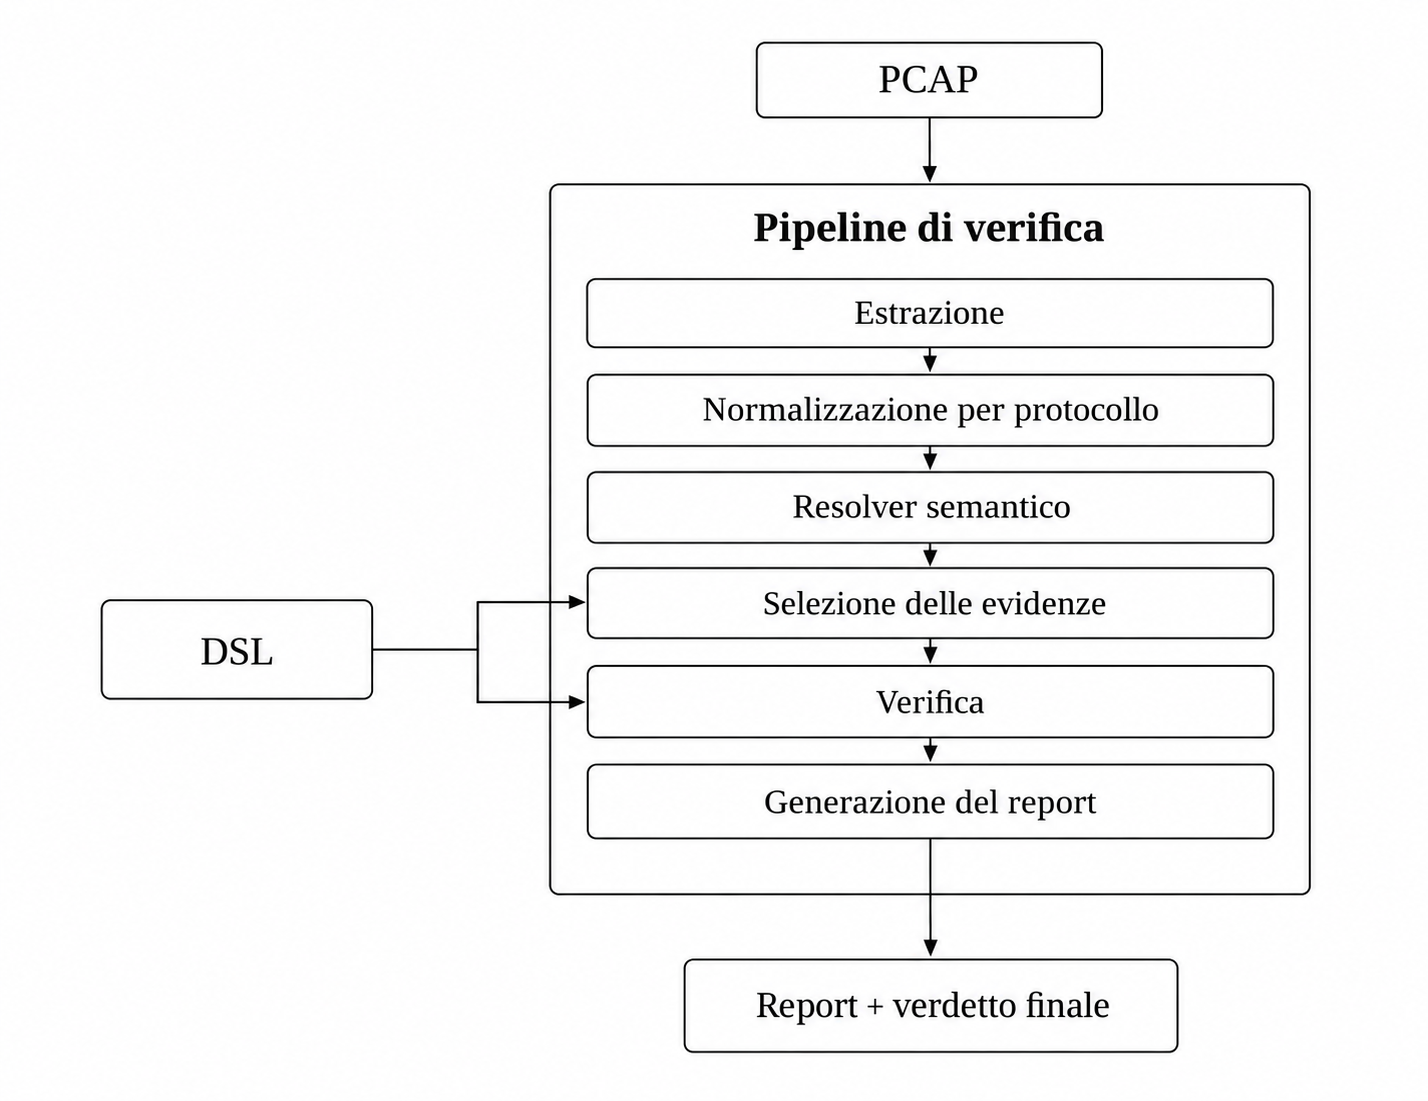
\includegraphics[width=0.94\textwidth,height=0.74\textheight,keepaspectratio]{figure/architettura_generale.png}
\caption{Architettura generale della pipeline di verifica degli esiti SCAS.}
\label{fig:architettura}
\end{figure}
\needspace{5\baselineskip}


Il sistema riceve due input principali: una cattura di traffico, contenente le evidenze da analizzare, e una specifica DSL, che definisce quali eventi individuare e quali condizioni verificare. Quest'ultima riveste un ruolo centrale nell'architettura, poiché guida la selezione delle evidenze e la successiva applicazione dei criteri, mentre la pipeline mette a disposizione i meccanismi comuni di elaborazione e verifica.

L'esecuzione è organizzata attraverso il file di configurazione \texttt{tests.json}, che associa a ciascun caso di test la cattura, la specifica DSL e i parametri necessari all'analisi. La Figura~\ref{fig:architettura} illustra l'organizzazione generale dell'architettura e le relazioni tra i suoi componenti.


\section{Estrazione strutturata del traffico}\label{estrazione-strutturata-del-traffico}

La cattura del traffico di rete effettuata durante un test viene conservata in un file PCAP, che costituisce la sorgente delle evidenze osservabili. Poiché le informazioni registrate non sono immediatamente disponibili in una forma adatta all'analisi, è necessaria una fase preliminare di estrazione che le renda accessibili in modo strutturato.

A tale scopo viene utilizzato TShark, un analizzatore di protocolli di rete che applica i \emph{dissector} dei protocolli presenti nella cattura e rende accessibili i relativi campi decodificati. L'estrazione avviene mediante l'opzione \texttt{-T\ ek}, che produce record strutturati in formato JSON, consentendo alla pipeline di operare sui campi decodificati anziché sui byte grezzi dei pacchetti. \cite{wireshark_tshark_docs}

I record prodotti contengono informazioni generali, come numero di frame, timestamp e indirizzi IP, insieme ai campi propri dei protocolli analizzati. La diversa organizzazione di questi campi rende necessaria una successiva fase di normalizzazione.

\section{Normalizzazione degli eventi}\label{normalizzazione-protocol-specifica}

La normalizzazione ha lo scopo di ricondurre le informazioni estratte dai diversi protocolli a una rappresentazione comune degli eventi di rete. Per ciascun protocollo supportato, un normalizzatore interpreta i campi disponibili e li organizza in un oggetto denominato \texttt{MessageEvent}, che raccoglie sia le informazioni generali dell'evento sia i dati specifici del messaggio.

La struttura del \texttt{MessageEvent} comprende i seguenti attributi:

\par\noindent\begin{minipage}{\linewidth}
\begin{lstlisting}
class MessageEvent:
    frame_number: int
    timestamp: float
    protocol: str
    kind: str
    
    src: str | None = None
    dst: str | None = None
    
    message_type: str | None = None
    
    related_frames: list[int] = field(default_factory=list)
    
    correlation: dict[str, Any] = field(default_factory=dict)
    
    fields: dict[str, Any] = field(default_factory=dict)
\end{lstlisting}
\end{minipage}\par

Nell'implementazione attuale sono previsti normalizzatori per NAS, HTTP/2 e PFCP.
\section{Risoluzione semantica}\label{risoluzione-semantica}

La normalizzazione produce eventi rappresentati secondo una struttura comune, ma in alcuni casi il loro significato applicativo non è ancora completamente esplicito. Ciò avviene soprattutto per messaggi relativi alle interazioni della Service-Based Architecture, dove i messaggi HTTP/2 possono rappresentare operazioni differenti in funzione del servizio richiesto e del contenuto applicativo.

Per gestire questa esigenza, viene introdotto un \emph{resolver semantico}, incaricato di interpretare gli eventi normalizzati e associarli a tipologie coerenti con il dominio 5G. Ad esempio, analizzando il percorso della richiesta HTTP/2, il resolver può riconoscere un'operazione di \emph{NF Discovery} presso l'NRF e classificare gli eventi correlati come \texttt{nrf.discovery.request} e \texttt{nrf.discovery.response}.

Il resolver opera quindi a un livello di astrazione superiore rispetto ai normalizzatori, in quanto non ricostruisce nuovamente i messaggi, ma utilizza le informazioni già disponibili per completarne l'interpretazione e rendere esplicito il tipo semantico degli eventi.

\section{Selezione dell'evidenza tramite DSL}\label{selezione-dellevidenza-tramite-dsl}

La normalizzazione e l'eventuale risoluzione semantica trasformano il traffico acquisito in una sequenza di eventi strutturati, tra i quali la fase di selezione individua quelli richiesti dal caso di test considerato.

Per descrivere le evidenze da individuare, il DSL mette a disposizione due costrutti principali: \texttt{SEQUENCE}, che permette di specificare una successione ordinata di eventi, e \texttt{COLLECT}, utilizzato per raccogliere più occorrenze di un determinato tipo di evento. Attraverso questi costrutti è possibile indicare quali eventi ricercare nella cattura e, quando necessario, le relazioni di ordine che devono sussistere tra essi.

Gli eventi individuati vengono associati a identificatori simbolici, denominati \emph{alias}, definiti nella specifica DSL. Un alias può rappresentare, ad esempio, un particolare messaggio riconosciuto tramite \texttt{SEQUENCE} oppure una collezione di messaggi ottenuta mediante \texttt{COLLECT}. L'associazione tra l'alias e l'evidenza corrispondente prende il nome di \emph{binding}.

I binding prodotti dalla selezione vengono raccolti nel \texttt{BindingContext}, una struttura che rende disponibili le evidenze individuate attraverso i rispettivi alias. I criteri di verifica possono così riferirsi direttamente agli eventi selezionati, indipendentemente dalla loro posizione nella cattura.


\section{Verifica}
\label{verifica}

Una volta costruito il \texttt{BindingContext}, la fase di verifica valuta l'evidenza selezionata rispetto ai criteri definiti nella DSL, al fine di stabilire se il comportamento osservato soddisfi le condizioni previste per il caso di test.

L'architettura prevede due modalità complementari: la verifica statica e la verifica temporale.

La prima opera sui valori associati ai binding, valutando proprietà e relazioni tra i dati estratti dagli eventi selezionati. È utilizzata, ad esempio, per controllare la corrispondenza tra valori o l'assenza di duplicati.

La seconda riguarda invece le relazioni temporali tra gli eventi, come il rispetto di determinati intervalli di tempo. Tali proprietà sono espresse mediante la \emph{Metric First-Order Temporal Logic} (MFOTL) e valutate attraverso il motore di verifica esterno MonPoly.

I risultati ottenuti dalle due modalità concorrono alla determinazione del verdetto complessivo del caso di test.


\section{Reporting}\label{reporting}

L'ultima fase dell'architettura riguarda la produzione del report, che affianca al verdetto le informazioni su cui esso si basa. Il reporter, comune ai diversi casi di test, organizza tali informazioni in un documento strutturato in formato \texttt{JSON}, distinguendo i dati relativi al test e all'esecuzione dai criteri valutati, dalle evidenze osservate e dal risultato complessivo.

\Needspace{16\baselineskip}
Il seguente schema illustrativo semplificato presenta i principali campi del report; i segnaposto indicano parti omesse e non costituiscono un documento JSON completo:

\par\noindent\begin{minipage}{\linewidth}
\begin{lstlisting}
{
    "metadata": {
        "generator": "generic_verification_pipeline",
        "tshark_version": "..."
    },
    "test": { "id": "..." },
    "source": { "pcap": "...", "sha256": "..." },
    "configuration": {
        "pipeline": "...", "rules": "...", "traffic": { }
    },
    "criteria": [ ... ],
    "verification": {
        "results": [ ... ],
        "overall_verdict": "PASS"
    },
    "evidence": { "bindings": { ... } },
    "explanation": { "summary": "..." },
    "verdict": "PASS"
}
\end{lstlisting}
\end{minipage}\par

Il report favorisce sia la verificabilità sia la riproducibilità dell'analisi. I criteri valutati e i riferimenti alle evidenze consentono di controllare le motivazioni del verdetto, mentre i metadati relativi alla cattura, alla configurazione e alla versione di TShark documentano alcune condizioni utili per ripetere la verifica. In particolare, l'hash SHA-256 del file PCAP permette di controllare che una successiva analisi utilizzi la stessa cattura.

% Capitolo 5 generato dalla bozza Markdown verificata.
\chapter{Domain-Specific Language e motore di verifica}\label{domain-specific-language-e-motore-di-verifica}

\section{Struttura della grammatica}\label{struttura-della-grammatica}

La sintassi del DSL è definita mediante una grammatica realizzata con Lark, una libreria Python per la costruzione di parser a partire da grammatiche formali. Le regole del linguaggio utilizzano i tipi semantici degli eventi e i relativi attributi, resi disponibili dalle fasi di normalizzazione e risoluzione semantica.

Una specifica è composta da istruzioni dedicate alla selezione delle evidenze e alla definizione dei criteri di verifica. La selezione può essere espressa attraverso \texttt{SEQUENCE}, che descrive una successione ordinata di eventi, oppure \texttt{COLLECT}, che raccoglie le occorrenze di un determinato tipo di evento. In entrambi i casi, la parola chiave \texttt{AS} permette di associare un identificatore simbolico, denominato alias, all'evidenza individuata. All'interno di \texttt{SEQUENCE} è inoltre possibile utilizzare \texttt{OPTIONAL} per indicare porzioni della sequenza la cui presenza non è obbligatoria.

I criteri di verifica sono definiti mediante \texttt{REQUIRE}, che consente di esprimere confronti tra valori letterali e campi degli eventi selezionati. Il linguaggio prevede inoltre \texttt{REQUIRE UNIQUE} per verificare proprietà di unicità e \texttt{IF} per applicare determinate regole soltanto quando una condizione è soddisfatta. Le proprietà temporali sono invece espresse mediante MFOTL.

\Needspace{19\baselineskip}
Le principali produzioni della grammatica sono riportate di seguito.

\par\noindent\begin{minipage}{\linewidth}
\begin{lstlisting}
start: statement+

?statement: sequence_rule
          | collect_rule
          | rule

?rule: static_rule
     | temporal_rule

?static_rule: comparison_rule
            | unique_rule
            | if_rule

sequence_rule: "SEQUENCE" "{" sequence_element+ "}"
?sequence_element: sequence_item | optional_block
sequence_item: FIELD "AS" NAME
optional_block: "OPTIONAL" "{" sequence_element+ "}"

collect_rule: "COLLECT" FIELD "AS" NAME

comparison_rule: "REQUIRE" FIELD OP operand
unique_rule: "REQUIRE" "UNIQUE" FIELD
if_rule: "IF" FIELD OP operand "{" rule+ "}"

temporal_rule: "MFOTL" "CASE" VALUE MFOTL_BLOCK

?operand: FIELD -> field_operand
        | VALUE -> literal_operand
\end{lstlisting}
\end{minipage}\par

I riferimenti agli eventi e ai relativi attributi sono rappresentati attraverso \texttt{FIELD}, che utilizza una notazione gerarchica separata da punti. Nella parte dedicata alla selezione, ad esempio, è possibile dichiarare:

\par\noindent\begin{minipage}{\linewidth}
\begin{lstlisting}
SEQUENCE {
    ausf.authentication.response AS initial_vector
    nas.authentication_request AS auth_request
}
\end{lstlisting}
\end{minipage}\par

In questo esempio, i due eventi semantici vengono associati rispettivamente agli alias \texttt{initial\_vector} e \texttt{auth\_request}, attraverso i quali è possibile accedere ai relativi campi nelle successive regole di verifica:

\par\noindent\begin{minipage}{\linewidth}
\begin{lstlisting}
REQUIRE auth_request.rand == initial_vector.rand
\end{lstlisting}
\end{minipage}\par

\texttt{NAME} identifica gli alias introdotti dalla specifica, mentre \texttt{VALUE} rappresenta valori letterali utilizzabili nelle espressioni. 



\section{Rappresentazione interna delle regole}\label{rappresentazione-interna-delle-regole}

Le istruzioni scritte nel DSL devono essere interpretate dal sistema per poter essere utilizzate durante la selezione e la verifica delle evidenze. A questo scopo, il parser costruito con Lark analizza la specifica e ne riconosce le strutture sintattiche, che vengono successivamente trasformate in rappresentazioni interne attraverso un \texttt{Transformer}.

Il matcher e i verificatori non operano quindi direttamente sul testo della DSL, ma su rappresentazioni strutturate che conservano esclusivamente le informazioni necessarie all'elaborazione.

A seconda dello statement considerato, vengono mantenute informazioni differenti, quali il tipo di operatore, i riferimenti ai campi, gli alias, gli operandi di confronto, eventuali regole annidate e, nel caso di proprietà temporali, la relativa formula.

Ad esempio, una regola come

\par\noindent\begin{minipage}{\linewidth}
\begin{lstlisting}
REQUIRE auth_request.rand == initial_vector.rand
\end{lstlisting}
\end{minipage}\par

viene trasformata concettualmente in una struttura del tipo:

\par\noindent\begin{minipage}{\linewidth}
\begin{lstlisting}
field: auth_request.rand
operator: ==
expected:
    type: field
    value: initial_vector.rand
\end{lstlisting}
\end{minipage}\par

In questo modo viene mantenuta anche la distinzione tra un operando costituito da un valore letterale e un operando che rappresenta invece il riferimento a un altro campo della specifica.

Per il costrutto \texttt{SEQUENCE}, la rappresentazione ottenuta dal parsing viene ulteriormente trasformata in un \emph{Abstract Syntax Tree} (AST) dedicato alla descrizione del pattern sequenziale. I tipi di nodo attualmente necessari sono:

\begin{itemize}
\tightlist
\item
  \texttt{Sequence}, che rappresenta l'insieme ordinato degli elementi del pattern;
\item
  \texttt{Atom}, associato a un singolo tipo di evento atteso e al relativo alias;
\item
  \texttt{Optional}, utilizzato per racchiudere elementi la cui presenza è opzionale.
\end{itemize}

Ad esempio, la specifica

\par\noindent\begin{minipage}{\linewidth}
\begin{lstlisting}
SEQUENCE {
    event.a AS a
    OPTIONAL {
        event.b AS b
    }
    event.c AS c
}
\end{lstlisting}
\end{minipage}\par

può essere rappresentata concettualmente attraverso il seguente albero:

\begin{verbatim}
Sequence
├── Atom(event.a, a)
├── Optional
│   └── Atom(event.b, b)
└── Atom(event.c, c)
\end{verbatim}


È importante precisare che non tutti gli elementi della DSL vengono trasformati nello stesso AST. La struttura composta da \texttt{Sequence}, \texttt{Atom} e \texttt{Optional} è specificamente utilizzata per rappresentare i pattern sequenziali, mentre le regole statiche e temporali vengono mantenute in strutture interne adatte ai rispettivi meccanismi di verifica.

Le rappresentazioni ottenute costituiscono quindi il livello di collegamento tra il parsing della specifica e i componenti incaricati della sua elaborazione.

Prima di procedere alla selezione dell'evidenza, viene inoltre effettuata una validazione strutturale degli alias utilizzati nei criteri statici. Questo controllo è necessario per verificare la coerenza dei riferimenti presenti nella specifica DSL, evitando che un alias utilizzato nelle regole di verifica, ma mai dichiarato, venga erroneamente interpretato come un'evidenza mancante durante l'analisi della cattura.

La validazione viene effettuata raccogliendo tutti gli alias dichiarati nella fase di selezione, a cui vengono aggiunti gli eventuali alias esterni, di configurazione o derivati. Questi vengono confrontati con gli alias utilizzati nelle regole di verifica, comprese le condizioni e le regole annidate. 

La validazione permette quindi di individuare gli alias utilizzati senza essere stati dichiarati, distinguendo gli errori presenti nella specifica dai casi in cui un alias correttamente dichiarato non risulti associato ad alcuna evidenza durante la selezione.


\section{Selezione mediante SEQUENCE}\label{selezione-mediante-sequence}

Questa sezione descrive il meccanismo utilizzato per individuare, all'interno del traffico osservato, le sequenze di eventi.

\subsection{Dal pattern all'automa}\label{il-pattern-sequenziale}

Per il riconoscimento dei pattern sequenziali, il sistema utilizza un automa a stati finiti non deterministico (\emph{Nondeterministic Finite Automaton}, NFA). Il pattern, precedentemente rappresentato mediante un AST, viene trasformato in un NFA che descrive i possibili percorsi di riconoscimento degli eventi.

Questa scelta permette di utilizzare un unico meccanismo di ricerca per sequenze con strutture differenti, comprese quelle contenenti blocchi \texttt{OPTIONAL}, senza dover sviluppare una logica di riconoscimento specifica per ciascun pattern.

\subsection{Formalizzazione dell'automa}\label{formalizzazione-dellautoma}

Formalmente, l'NFA adottato è definito dalla seguente quintupla:
\[
A = \langle \Sigma, \ Q, \ q_{0}, \ Q_{F}, \ \delta \rangle
\] dove

\begin{itemize}
\tightlist
\item
  \(\Sigma\) è l'alfabeto, costituito dall'insieme dei tipi semantici di evento riconosciuti dall'automa;
\item
  \(Q\) è l'insieme finito degli stati;
\item
  \(q_{0} \in Q\) è lo stato iniziale;
\item
  \(Q_{F} \subseteq Q\) è l'insieme degli stati finali. Nell'implementazione proposta viene utilizzato un unico stato di accettazione, pertanto \(Q_{F} = \{ q_{f} \}\);
\item
  \(\delta\) è la funzione di transizione non deterministica, definita come \[\delta: Q \times (\Sigma \ \cup \ \{  \varepsilon \}) \to \mathcal{P}(Q)\]
\end{itemize}

dove \(\mathcal{P}(Q) = 2^{Q}\) indica l'insieme delle parti di \(Q\), ossia l'insieme di tutti i suoi sottoinsiemi.



\subsection{\texorpdfstring{Le \(\varepsilon\)-transizioni}{Le \textbackslash varepsilon-transizioni}}\label{le-varepsilon-transizioni}

Una transizione ordinaria, etichettata con un simbolo \(a \in \Sigma\), può essere attraversata soltanto quando l'evento corrente della traccia presenta il tipo semantico richiesto. Il suo attraversamento comporta il consumo dell'evento e l'avanzamento nella lettura della traccia. Tale transizione è rappresentata come:

\[
q_{i} \xrightarrow{a} q_{j}
\]

Una transizione \(\varepsilon\), invece, ha la forma:

\[
q_{i} \xrightarrow{\varepsilon} q_{j}
\] e permette di passare da uno stato all'altro senza consumare alcun evento, ossia senza avanzare nella lettura della traccia.

Le \(\varepsilon\)-transizioni permettono quindi di collegare stati e percorsi dell'automa senza richiedere il riconoscimento di nuovi eventi. Questa caratteristica viene utilizzata nella costruzione di Thompson per combinare i diversi frammenti che compongono il pattern. 

\subsection{Compilazione del pattern mediante Thompson}\label{compilazione-del-pattern-mediante-thompson}

Una volta ottenuto l'AST, il pattern sequenziale viene compilato in un NFA mediante la costruzione di Thompson \cite{thompson_1968}. Tale procedimento si basa su un approccio composizionale: a ciascun nodo dell'albero viene associato un frammento dell'automa, dotato di uno stato iniziale e uno finale; i frammenti vengono successivamente collegati per ottenere l'automa corrispondente alla sequenza completa.

La costruzione dipende dal tipo di nodo considerato:

\begin{itemize}
\tightlist
\item
  \texttt{Atom}: genera un frammento costituito da due stati collegati da una transizione etichettata con il tipo semantico dell'evento atteso.
\item
  \texttt{Sequence}: combina i frammenti dei propri elementi nell'ordine specificato, collegando lo stato finale di ciascun frammento allo stato iniziale del successivo mediante una transizione \(\varepsilon\).
\item
  \texttt{Optional}: il blocco viene rappresentato mediante due percorsi alternativi collegati da transizioni \(\varepsilon\): uno attraversa il frammento corrispondente agli eventi opzionali, mentre l'altro consente di saltarlo senza consumare tali eventi.
\end{itemize}

Considerando il pattern sequenziale già introdotto nella Sezione~\ref{rappresentazione-interna-delle-regole}, la Figura~\ref{fig:thompson} ne mostra una rappresentazione schematica mediante NFA, ottenuta applicando la costruzione di Thompson ai nodi dell'AST.

\begin{figure}[H]
    \centering
    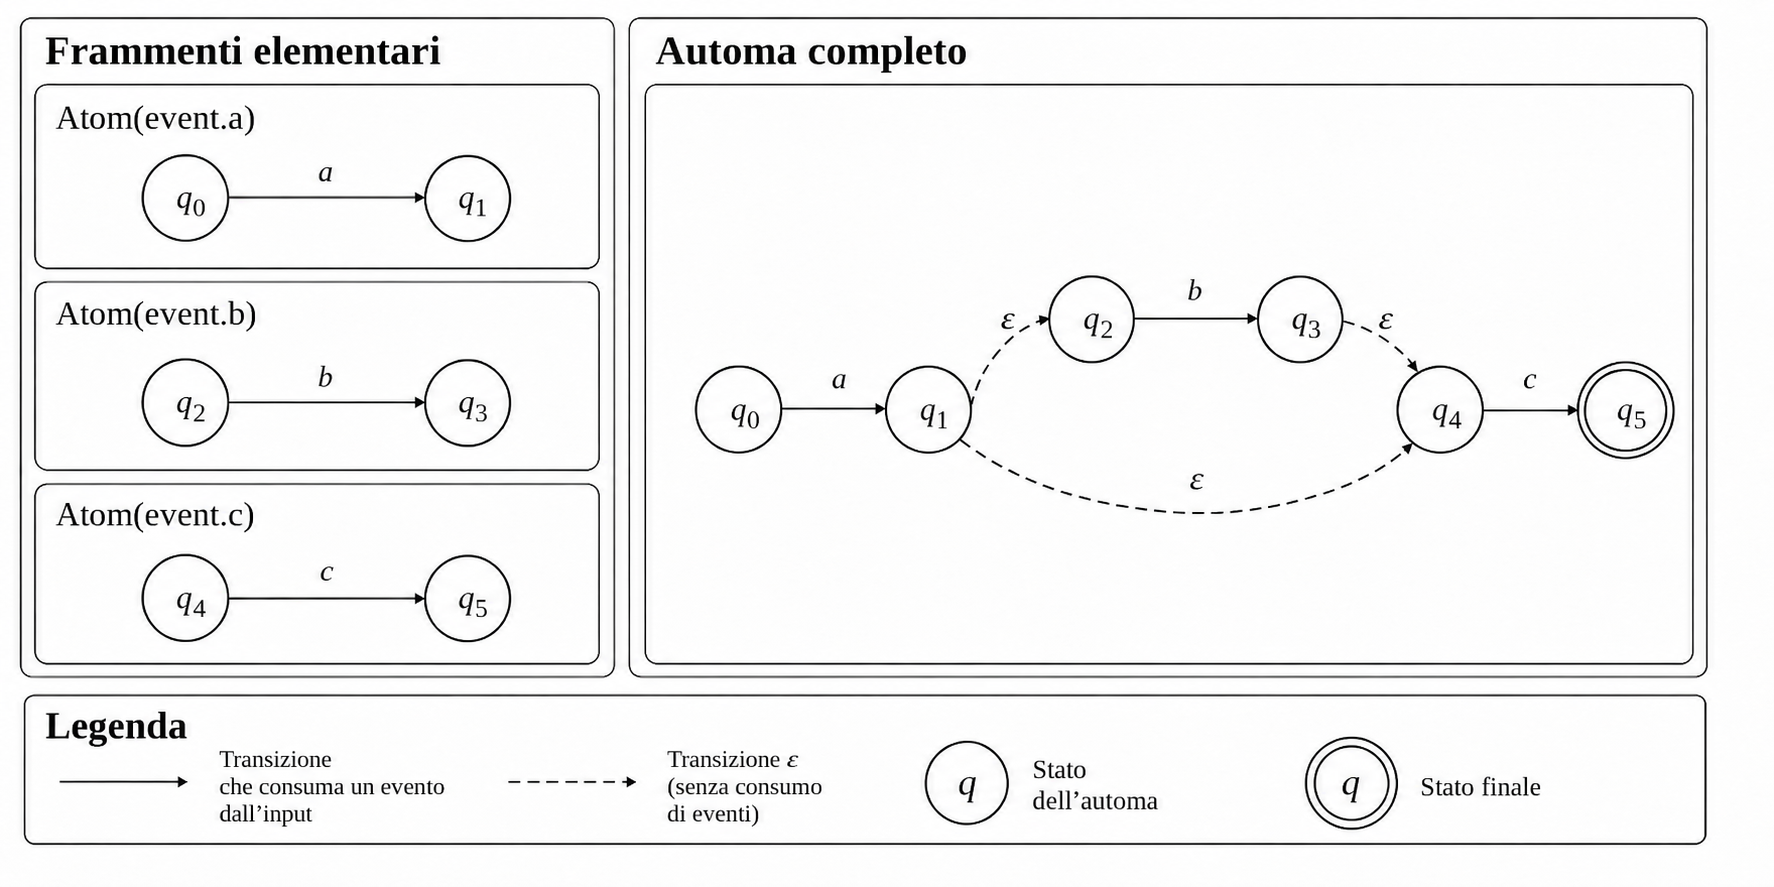
\includegraphics[
        width=\textwidth,
        height=0.65\textheight,
        keepaspectratio
    ]{figure/nfa_thompson.png}
    \caption{Rappresentazione schematica semplificata di un NFA per una sequenza contenente un blocco opzionale.}
    \label{fig:thompson}
\end{figure}

\subsection{Funzionamento del matcher}\label{configurazioni-attive-e-riconoscimento-degli-eventi}

Il riconoscimento delle sequenze di eventi all'interno della traccia è affidato al matcher, il componente che utilizza l'NFA per individuare le corrispondenze con il pattern definito nella DSL. Il matcher riceve in ingresso l'automa e la sequenza ordinata di \texttt{MessageEvent}, esaminando gli eventi per individuare i percorsi che consentono di raggiungere uno stato accettante.

Durante questa operazione non è sufficiente conoscere lo stato raggiunto nell'automa, poiché è necessario conservare anche i riferimenti agli eventi che hanno contribuito al riconoscimento. A questo scopo viene introdotta una struttura denominata \texttt{ActiveConfiguration}, formalizzabile come:

\[
C = \langle q, B \rangle
\]

dove

\begin{itemize}
\tightlist
\item
  \(q \in Q\) è lo stato corrente dell'automa;
\item
  \(B\) è una funzione parziale che associa gli alias definiti nella DSL ai \texttt{MessageEvent} già riconosciuti.
\end{itemize}

Il matcher può mantenere contemporaneamente più configurazioni attive, ciascuna caratterizzata dal proprio stato e dai binding progressivamente costruiti.

Poiché l'automa può contenere transizioni \(\varepsilon\), per ogni stato corrente devono essere considerati anche quelli raggiungibili senza consumare ulteriori eventi. A tale scopo viene utilizzata una \(\varepsilon \text{-closure}\), definita formalmente come:

\[
\varepsilon\text{-closure}(q) = \{ p \in Q \mid q \xrightarrow{ \ \ \varepsilon^{*} \ } p\}
\]

La chiusura comprende tutti gli stati raggiungibili da \(q\) attraverso zero o più transizioni \(\varepsilon\), incluso lo stesso \(q\). L'espansione di una configurazione attraverso tali transizioni mantiene invariati i binding già acquisiti, poiché non viene riconosciuto alcun nuovo evento.

Durante la scansione della traccia, il matcher confronta il \texttt{message\_type} di ciascun evento con quello richiesto dalle transizioni uscenti dagli stati delle configurazioni attive. Quando viene individuata una transizione compatibile, la configurazione avanza verso lo stato di destinazione e il \texttt{MessageEvent} osservato viene associato all'alias definito nel corrispondente \texttt{Atom}. I binding vengono quindi aggiornati e vengono considerate le ulteriori transizioni \(\varepsilon\) raggiungibili dal nuovo stato.

Una caratteristica importante è che la selezione non richiede che gli eventi previsti dal pattern siano consecutivi nella traccia. Quando un evento non può essere consumato da una determinata configurazione, quest'ultima può rimanere attiva, consentendo di proseguire la ricerca con gli eventi successivi.

La possibilità di mantenere più configurazioni attive consente inoltre al matcher di seguire simultaneamente le alternative previste dall'NFA in presenza di blocchi \texttt{OPTIONAL}, comprese le configurazioni raggiungibili mediante \(\varepsilon\)-transizioni che consentono di omettere gli eventi opzionali.

\subsection{Avvio e riavvio dei candidati}\label{politica-di-matching-e-produzione-dei-risultati}

All'interno di una cattura possono essere presenti più occorrenze degli eventi descritti dalla stessa \texttt{SEQUENCE}, anche in posizioni differenti della traccia. Il matcher esamina quindi gli eventi in ordine e, per ogni posizione compatibile con l'inizio del pattern, avvia un nuovo candidato di riconoscimento. Ciascun candidato rappresenta un tentativo indipendente di completare la sequenza a partire dalla posizione individuata e può mantenere più configurazioni attive, corrispondenti ai diversi percorsi dell'automa.

Durante l'elaborazione viene applicata una politica di riavvio (\emph{restart policy}), finalizzata a evitare che eventi appartenenti a tentativi distinti vengano associati alla stessa sequenza. Se viene incontrato un evento compatibile con l'inizio di un nuovo candidato, ma che non può essere consumato da nessuna delle configurazioni attive del candidato corrente, quest'ultimo viene interrotto. L'evento potrà comunque essere considerato come punto di partenza di un candidato distinto.

\subsection{Produzione e filtraggio dei match}\label{produzione-e-filtraggio-dei-match}

Un candidato completa il riconoscimento quando almeno una delle sue configurazioni raggiunge lo stato accettante dell'NFA. Per ciascun candidato viene considerato il primo punto di completamento, nel quale possono tuttavia essere presenti più configurazioni accettanti, associate a percorsi differenti dell'automa.

A ogni configurazione accettante corrisponde un oggetto \texttt{Match}, che conserva la posizione iniziale del candidato (\texttt{start\_index}), quella in cui è stato completato il riconoscimento (\texttt{end\_index}) e i binding degli eventi individuati. Il matcher può quindi produrre più match, anche a partire da uno stesso candidato.

La presenza di percorsi alternativi, in particolare quelli introdotti da \texttt{OPTIONAL}, può produrre match riferiti allo stesso intervallo della traccia ma contenenti binding differenti. Per eliminare i risultati meno completi senza perdere evidenze distinte, viene applicato un criterio di dominanza: un match domina un altro quando sono soddisfatte tutte le seguenti condizioni.

\begin{itemize}
\tightlist
\item
  i due match condividono \texttt{start\_index} e \texttt{end\_index};
\item
  gli alias del secondo costituiscono un sottoinsieme proprio di quelli del primo;
\item
  per tutti gli alias comuni, le associazioni fanno riferimento agli stessi eventi osservati.
\end{itemize}

Il filtraggio elimina quindi soltanto i match dominati, conservando quelli che presentano associazioni differenti o che non sono confrontabili secondo tali condizioni.

Al termine del filtraggio, il matcher restituisce i match completi non dominati, che costituiscono il risultato della selezione sequenziale e contengono le associazioni tra gli alias e gli eventi riconosciuti.

\section{Selezione mediante COLLECT}\label{selezione-mediante-collect}

La selezione mediante \texttt{COLLECT} viene effettuata confrontando il tipo semantico dichiarato nella regola con il campo \texttt{message\_type} degli eventi disponibili. Tutte le occorrenze corrispondenti vengono raccolte e associate all'alias specificato, senza richiedere la costruzione di un automa.

Una regola di raccolta può essere espressa come segue:

\par\noindent\begin{minipage}{\linewidth}
\begin{lstlisting}
COLLECT pfcp.session_establishment_response AS responses
\end{lstlisting}
\end{minipage}\par

In questo esempio, \texttt{pfcp.session\_establishment\_response} identifica il tipo di evento da ricercare, mentre \texttt{responses} è l'alias assegnato alla collezione risultante.

Gli eventi individuati vengono associati all'alias all'interno del \texttt{BindingContext}. A differenza di \texttt{SEQUENCE}, dove ciascun alias identifica un singolo evento riconosciuto, nel caso di \texttt{COLLECT} il valore associato è una lista di \texttt{MessageEvent}, rappresentabile come:

\[
B(\texttt{responses}) = [e_1, e_2, e_3, ..., e_n]
\] La struttura del \texttt{BindingContext} rimane quindi invariata, mentre cambia la natura dell'evidenza associata all'alias. Le due modalità di selezione, pur adottando meccanismi differenti, producono così una rappresentazione comune dei risultati.

\section{Verifica statica}\label{verifica-statica}

Il verificatore statico utilizza i binding presenti nel \texttt{BindingContext} per valutare i criteri definiti nelle regole DSL. Per effettuare le verifiche, riceve il contesto prodotto dalla selezione e le regole ottenute durante il parsing della specifica.

\Needspace{7\baselineskip}
Le regole di confronto sono introdotte dalla parola chiave \texttt{REQUIRE} e possono essere espresse nella forma generale:

\par\noindent\begin{minipage}{\linewidth}
\begin{lstlisting}
REQUIRE alias.campo OP valore
\end{lstlisting}
\end{minipage}\par

dove OP identifica l'operatore di confronto, mentre l'operando a destra può essere un valore letterale oppure un riferimento a un altro campo.

Per effettuare la valutazione, il verificatore deve innanzitutto risolvere i riferimenti presenti nella regola. Nel caso di un binding associato a un singolo evento, viene individuato l'alias interno del \texttt{BindingContext} e recuperato il relativo \texttt{MessageEvent}. Il percorso gerarchico specificato nella DSL viene quindi utilizzato per accedere ai campi, anche annidati, contenuti nell'attributo \texttt{fields} dell'evento. Quando invece il binding contiene una collezione, il campo richiesto viene recuperato da ciascuna evidenza, conservando anche il riferimento ai frame da cui proviene. Il medesimo meccanismo consente inoltre di accedere a informazioni esterne o derivate, eventualmente aggiunte al \texttt{BindingContext}, attraverso gli stessi riferimenti gerarchici utilizzati per gli eventi selezionati.

Una volta risolti i riferimenti presenti nella regola, il verificatore dispone dei valori necessari per applicare il criterio richiesto. La valutazione può consistere nel confronto tra due valori oppure nel controllo dell'unicità degli elementi di una collezione. In quest'ultimo caso, vengono considerate anche informazioni strutturate o contenenti più valori, conservando i riferimenti ai frame degli eventuali duplicati individuati.

La valutazione può inoltre dipendere da una condizione definita mediante \texttt{IF}. Quando la condizione è soddisfatta, il verificatore esegue le regole contenute nel blocco; in caso contrario, queste non vengono valutate e il blocco assume lo stato \texttt{SKIPPED}. Tale stato indica che le verifiche condizionali non sono applicabili e non rappresenta un ulteriore verdetto del test.

Ogni criterio valutato produce un risultato strutturato che associa l'esito alle informazioni utilizzate nella verifica, come i valori osservati e attesi e, quando pertinenti, i riferimenti ai frame. Questi risultati costituiscono la base per la successiva determinazione del verdetto complessivo.

\section{Verifica temporale}\label{verifica-temporale}

La verifica temporale permette di valutare proprietà che dipendono non soltanto dai valori contenuti nei messaggi, ma anche dalle relazioni temporali tra gli eventi osservati. A questo scopo viene utilizzata la \emph{Metric First-Order Temporal Logic} (MFOTL) \cite{basin_mfotl_2015}, un formalismo che consente di esprimere proprietà mediante predicati e operatori temporali, associando a questi ultimi intervalli entro cui devono essere soddisfatte determinate condizioni.

Le formule vengono valutate attraverso MonPoly \cite{basin_monpoly_2017}, un motore di monitoraggio esterno che verifica proprietà MFOTL su tracce temporizzate. La formula descrive quindi la proprietà richiesta, mentre MonPoly ne valuta il soddisfacimento rispetto agli eventi osservati.

\Needspace{10\baselineskip}
All'interno del DSL, una proprietà temporale può essere dichiarata mediante il costrutto \texttt{MFOTL CASE}. Il seguente esempio, tratto dal test AMF Synchronization Failure -- Case A, richiede che a una richiesta di risincronizzazione segua una risposta AUSF entro un intervallo temporale configurato.

\par\noindent\begin{minipage}{\linewidth}
\begin{lstlisting}
MFOTL CASE A """
ResynchronizationRequest()
IMPLIES
EVENTUALLY[0,{TIMER_MS}] AusfAuthenticationResponse()
"""
\end{lstlisting}
\end{minipage}\par

Per valutare la formula, MonPoly richiede una traccia temporizzata, nella quale gli eventi sono rappresentati mediante predicati associati ai rispettivi timestamp. Il sistema costruisce questa traccia a partire dagli eventi riconosciuti durante la selezione, utilizzando la configurazione del test per stabilire la corrispondenza tra gli alias della DSL e i predicati della formula.

La stessa configurazione indica il file di \emph{signature}, nel quale sono dichiarati i nomi dei predicati e gli eventuali argomenti che MonPoly può riconoscere. Nell'esempio precedente, tra i predicati utilizzati figurano \texttt{ResynchronizationRequest()} e \texttt{AusfAuthenticationResponse()}. Prima dell'esecuzione, il parametro \texttt{\{TIMER\_MS\}} viene sostituito con il valore configurato per il test, espresso in millisecondi.

Una volta preparate la formula, la signature e la traccia temporizzata, il sistema avvia MonPoly per effettuare la verifica. Nell'implementazione sviluppata viene utilizzata l'opzione \texttt{-negate}, che consente di monitorare la negazione della proprietà specificata e quindi di individuare le eventuali violazioni della formula originale. L'output prodotto da MonPoly viene infine interpretato dal verificatore per determinare l'esito del controllo temporale.

\section{Determinazione del verdetto}\label{determinazione-del-verdetto}

Il risultato della verifica di un caso di test è espresso attraverso uno dei tre verdetti previsti dal sistema: \texttt{PASS}, quando i criteri richiesti risultano soddisfatti; \texttt{FAIL}, quando viene rilevata una violazione; e \texttt{INCONCLUSIVE}, quando le evidenze disponibili non consentono di determinare un esito conclusivo.

Il verdetto \texttt{INCONCLUSIVE} viene prodotto quando le evidenze disponibili non consentono di valutare in modo conclusivo i criteri del caso di test. Questa situazione può verificarsi già durante la selezione: nel caso di \texttt{SEQUENCE}, quando non viene individuato alcun match completo oppure quando, anche dopo il filtraggio, rimangono più corrispondenze complete; nel caso di \texttt{COLLECT}, quando non sono presenti eventi del tipo semantico richiesto. L'impossibilità di concludere la verifica può emergere anche successivamente, qualora un criterio statico applicabile richieda un alias al quale non è stato associato alcun evento, come può accadere per un blocco \texttt{OPTIONAL} non attraversato durante il riconoscimento. In quest'ultimo caso, il verificatore non dispone dei valori necessari per valutare la regola: l'assenza dell'evidenza richiesta non permette di stabilire né il soddisfacimento né la violazione del criterio.

\Needspace{18\baselineskip}
Quando il caso di test prevede più criteri di verifica, i rispettivi risultati vengono combinati secondo una logica a tre valori, riportata nella Tabella~\ref{tab:aggregazione-tre-valori}.

\begin{center}
\begin{minipage}{0.88\textwidth}
\centering
\begingroup
\small
\renewcommand{\arraystretch}{1.18}
\begin{tabularx}{\linewidth}{|>{\centering\arraybackslash}X|>{\centering\arraybackslash}X|>{\centering\arraybackslash}X|}
\hline
\rowcolor{blue!7}
\textbf{Criterio A} & \textbf{Criterio B} & \textbf{Risultato} \\
\hline
PASS & PASS & PASS \\
\hline
PASS & FAIL & FAIL \\
\hline
PASS & INCONCLUSIVE & INCONCLUSIVE \\
\hline
FAIL & PASS & FAIL \\
\hline
FAIL & FAIL & FAIL \\
\hline
FAIL & INCONCLUSIVE & FAIL \\
\hline
INCONCLUSIVE & PASS & INCONCLUSIVE \\
\hline
INCONCLUSIVE & FAIL & FAIL \\
\hline
INCONCLUSIVE & INCONCLUSIVE & INCONCLUSIVE \\
\hline
\end{tabularx}
\endgroup
\captionof{table}{Tabella di aggregazione dei risultati di verifica secondo una logica a tre valori.}
\label{tab:aggregazione-tre-valori}
\end{minipage}
\end{center}

Come mostrato nella Tabella~\ref{tab:aggregazione-tre-valori}, il verdetto complessivo è \texttt{PASS} quando tutti i criteri applicabili risultano soddisfatti e \texttt{FAIL} quando almeno uno di essi rileva una violazione. \texttt{INCONCLUSIVE} viene invece prodotto quando non sono state rilevate violazioni, ma almeno un criterio non può essere valutato. Le regole contrassegnate come \texttt{SKIPPED} sono escluse dall'aggregazione, poiché non applicabili.

La stessa logica viene utilizzata quando il caso di test prevede sia verifiche statiche sia temporali, combinando i rispettivi risultati per determinare un unico verdetto complessivo.



% Capitolo 6 generato dalla bozza Markdown verificata.
\chapter{Testing e Mutation testing}\label{testing-e-mutation-testing}

\section{Obiettivi e metodologia della validazione}\label{obiettivi-e-metodologia-della-validazione}

La validazione sperimentale comprende sia i casi di test SCAS che hanno guidato lo sviluppo iniziale del sistema, sia ulteriori casi introdotti successivamente per ampliare e valutare le funzionalità supportate. Gli esperimenti considerano procedure relative a differenti funzioni della 5G Core Network, utilizzando come evidenza le informazioni ricavate dalle catture di traffico.

Sono inoltre previsti esperimenti di \emph{mutation testing} \cite{jia_harman_mutation_2011}, finalizzati a valutare la sensibilità del sistema ad alterazioni controllate dell'evidenza. La metodologia adottata e i relativi risultati sono approfonditi nella Sezione~\ref{mutation-testing}.

\section{Ambiente sperimentale e casi di test}\label{ambiente-sperimentale-e-casi-di-test}

Per la validazione sono stati utilizzati i seguenti ambienti e strumenti:

\begin{itemize}
\tightlist
\item
  Open5GS \cite{open5gs_docs}, implementazione open-source della 5G Core Network che fornisce le principali Network Functions previste dall'architettura 5G;
\item
  free5GC \cite{free5gc_docs}, implementazione open-source della 5G Core Network, utilizzabile per lo studio e la sperimentazione delle procedure e delle interazioni tra Network Functions;
\item
  ScasDK \cite{mancini_scasdk_2025}, piattaforma per l'esecuzione automatizzata di test di sicurezza SCAS, impiegata come riferimento sperimentale; alcuni suoi componenti sono stati adattati per le prove relative a NRF e UDM.
\end{itemize}

Il sistema proposto opera su catture di traffico già disponibili. L'esecuzione delle procedure SCAS e la generazione del traffico rimangono quindi distinte dalla verifica dell'esito e non rientrano tra le funzionalità della pipeline sviluppata, in accordo con il perimetro definito nella Sezione~\ref{scope-e-assunzioni}.

\Needspace{24\baselineskip}
I casi di test relativi alle funzioni NRF, UDM, AMF e UPF, definiti nelle rispettive specifiche SCAS \cite{3gpp_ts33518_2024,3gpp_ts33514_2021,3gpp_ts33512_2022,3gpp_ts33513_2023}, sono riepilogati nelle Tabelle~\ref{tab:open5gs_results} e~\ref{tab:free5gc_results}, organizzate in base all'implementazione della 5G Core Network da cui provengono le catture analizzate. Per ciascun caso vengono riportati il criterio di verifica applicato e il verdetto ottenuto.


\begin{center}
\begin{minipage}{\textwidth}
\centering

\begingroup
\small
\setlength{\tabcolsep}{5pt}
\renewcommand{\arraystretch}{1.3}

\begin{tabularx}{\linewidth}{|
    >{\raggedright\arraybackslash}p{0.31\linewidth}|
    >{\raggedright\arraybackslash}X|
    >{\centering\arraybackslash}p{0.19\linewidth}|}
\hline

\rowcolor{blue!7}
\textbf{Caso di test} &
\textbf{Criterio di verifica} &
\textbf{Verdetto} \\
\hline

NRF Discovery Authorization &
Risposta HTTP 403 &
FAIL \\
\hline

UDM Resynchronization &
Coerenza dei parametri di autenticazione &
PASS \\
\hline

UDM SUCI De-concealment &
SUPI restituito uguale al valore atteso &
PASS \\
\hline

AMF Sync Failure -- \mbox{Case A} &
Coerenza dei messaggi e \mbox{vincolo T3520} &
PASS \\
\hline

AMF Sync Failure -- \mbox{Case B} &
Coerenza dei messaggi e \mbox{vincolo T3520} &
PASS \\
\hline

UPF TEID Uniqueness &
Assenza di F-TEID duplicati &
PASS \\
\hline

AMF RES* -- Case A &
Gestione del fallimento di autenticazione &
PASS \\
\hline

AMF RES* -- Case B &
Gestione del fallimento di autenticazione &
\mbox{INCONCLUSIVE} \\
\hline

AMF RES* -- Case C &
Gestione del fallimento di autenticazione &
\mbox{INCONCLUSIVE} \\
\hline

AMF RES* -- Case D &
Gestione del fallimento di autenticazione &
\mbox{INCONCLUSIVE} \\
\hline

\end{tabularx}
\endgroup

\captionof{table}{Casi di test SCAS e verdetti ottenuti su Open5GS.}
\label{tab:open5gs_results}

\end{minipage}
\end{center}




\begin{center}
\begin{minipage}{\textwidth}
\centering

\begingroup
\small
\setlength{\tabcolsep}{5pt}
\renewcommand{\arraystretch}{1.3}

\begin{tabularx}{\linewidth}{|
    >{\raggedright\arraybackslash}p{0.31\linewidth}|
    >{\raggedright\arraybackslash}X|
    >{\centering\arraybackslash}p{0.19\linewidth}|}
\hline

\rowcolor{blue!7}
\textbf{Caso di test} &
\textbf{Criterio di verifica} &
\textbf{Verdetto} \\
\hline

AMF Sync Failure -- Case A &
Coerenza dei messaggi e vincolo T3520 &
PASS \\
\hline

AMF Sync Failure -- Case B &
Coerenza dei messaggi e vincolo T3520 &
PASS \\
\hline

AMF RES* -- Case A &
Gestione del fallimento di autenticazione &
PASS \\
\hline

AMF RES* -- Case B &
Gestione del fallimento di autenticazione &
PASS \\
\hline

AMF RES* -- Case C &
Gestione del fallimento di autenticazione &
PASS \\
\hline

AMF RES* -- Case D &
Gestione del fallimento di autenticazione &
PASS \\
\hline

\end{tabularx}
\endgroup

\captionof{table}{Casi di test SCAS e verdetti ottenuti su free5GC.}
\label{tab:free5gc_results}

\end{minipage}
\end{center}





I verdetti riportati rappresentano l'esito della verifica dei criteri dichiarati rispetto all'evidenza osservata. Un risultato \texttt{FAIL} non indica quindi necessariamente un malfunzionamento della pipeline, ma può corrispondere alla corretta rilevazione di un criterio non soddisfatto. È il caso del test NRF, nel quale la risposta osservata presenta uno status HTTP \texttt{200}, mentre la regola DSL richiede \texttt{403}.

\section{Valutazione delle capacità di verifica}\label{valutazione-delle-capacituxe0-di-verifica}

In questa sezione vengono approfonditi tre gruppi di casi di test, selezionati per esaminare il comportamento delle principali capacità di verifica implementate.

\subsection{AMF Synchronization Failure - Case B}\label{amf-synchronization-failure---case-b}

L'analisi di \texttt{AMF\ Synchronization\ Failure\ -\ Case\ B} coinvolge tre componenti del sistema: la selezione mediante \texttt{SEQUENCE}, la verifica statica sui campi degli eventi e la verifica temporale attraverso MonPoly.

Il caso riguarda la gestione di un fallimento di sincronizzazione durante la procedura di autenticazione 5G AKA. A seguito della ricezione di un'\texttt{Authentication\ Request}, l'UE segnala un \texttt{Authentication\ Failure} con causa di sincronizzazione e fornisce il parametro \texttt{AUTS} necessario alla risincronizzazione. L'AMF inoltra quindi le informazioni necessarie all'AUSF. Il timer NAS T3520, avviato dall'UE a seguito dell'invio dell'\texttt{Authentication\ Failure}, ha un valore di 15 secondi nelle condizioni ordinarie di accesso considerate \cite{3gpp_ts24501_2025}; tale intervallo è utilizzato come parametro di riferimento per il criterio temporale configurato nel test. Nel Case B, il criterio temporale verifica che, nell'intervallo configurato a partire dal fallimento di sincronizzazione, non venga osservata una nuova \texttt{Authentication\ Request} prima della risposta AUSF successiva alla richiesta di risincronizzazione.

\begin{figure}[!htbp]
\centering
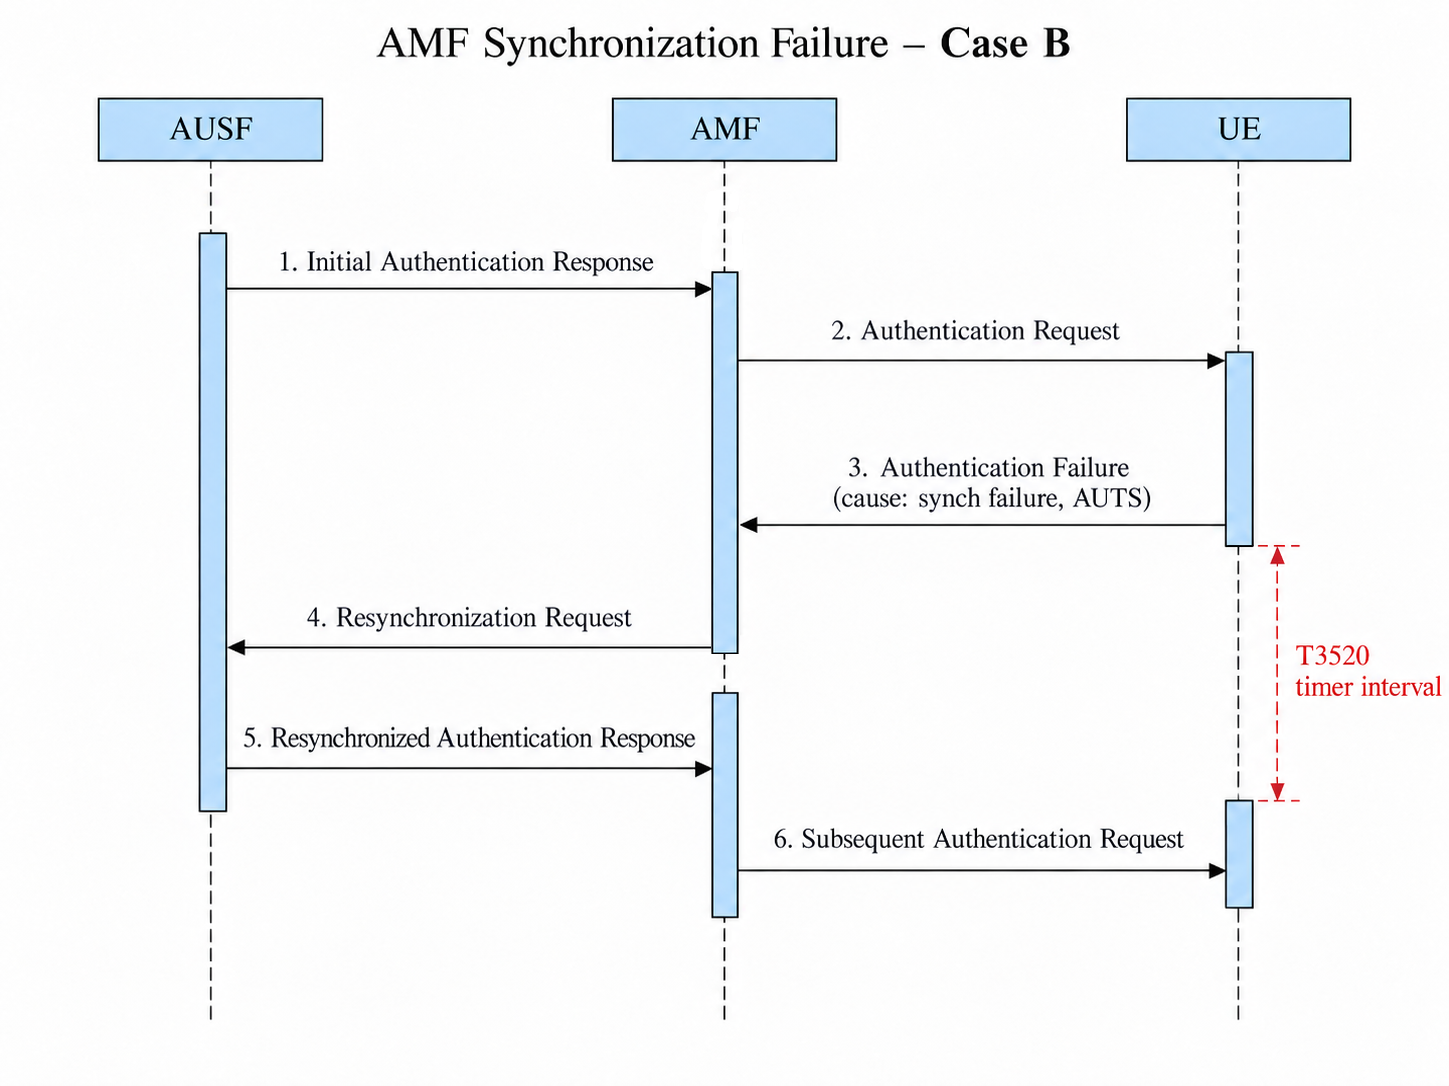
\includegraphics[width=0.94\textwidth,height=0.73\textheight,keepaspectratio]{figure/amf_sync_failure_case_b.png}
\caption{Scambio di messaggi nell'AMF Synchronization Failure, Case B, con vincolo temporale T3520.}
\label{fig:amf-sync-b}
\end{figure}

\Needspace{18\baselineskip}
La specifica DSL del caso descrive la successione degli eventi attesi e i criteri statici da valutare:

\par\noindent\begin{minipage}{\linewidth}
\begin{lstlisting}
SEQUENCE {
    ausf.authentication.response AS initial_vector
    nas.authentication_request AS initial_auth
    nas.authentication_failure AS sync_failure
    ausf.resynchronization.request AS resync
    ausf.authentication.response AS new_vector
    nas.authentication_request AS subsequent_auth_request
}

REQUIRE initial_auth.rand == initial_vector.rand
REQUIRE sync_failure.cause == 21
REQUIRE resync.auts == sync_failure.auts
REQUIRE resync.rand == initial_auth.rand
\end{lstlisting}
\end{minipage}\par

A questa si affianca la proprietà temporale MFOTL, che esclude la presenza di una nuova \texttt{Authentication\ Request} precedente alla risposta AUSF nell'intervallo configurato dopo il fallimento di sincronizzazione:

\par\noindent\begin{minipage}{\linewidth}
\begin{lstlisting}
MFOTL CASE B """
  SyncFailure()
  IMPLIES
  NOT (
      (NOT AusfAuthenticationResponse())
      UNTIL[0,{TIMER_MS}]
      AuthenticationRequest()
  )
"""
\end{lstlisting}
\end{minipage}\par

L'analisi delle catture provenienti da free5GC e Open5GS ha prodotto, in entrambi i casi, un unico match completo, associando agli alias dichiarati gli eventi individuati nel traffico. Le quattro verifiche statiche hanno restituito PASS per entrambe le implementazioni:

\begin{itemize}
\tightlist
\item
  corrispondenza del \texttt{RAND} tra risposta \texttt{AUSF} iniziale e l'Authentication Request;
\item
  presenza della causa \texttt{NAS\ 21} nell'Authentication Failure;
\item
  corrispondenza di \texttt{AUTS} tra l'Authentication Failure e la richiesta di risincronizzazione;
\item
  corrispondenza del \texttt{RAND} iniziale con quello utilizzato nella richiesta di risincronizzazione.
\end{itemize}

Anche la verifica temporale ha restituito PASS in entrambe le catture, sebbene siano stati osservati intervalli differenti tra i messaggi. In free5GC, l'Authentication Failure viene individuato al frame 358, mentre la successiva risposta AUSF e la nuova Authentication Request compaiono rispettivamente ai frame 604 e 606, circa 25 secondi dopo il fallimento di sincronizzazione. In Open5GS, gli stessi eventi vengono individuati ai frame 276, 432 e 434, con un intervallo di circa 11 secondi tra l'Authentication Failure e la nuova Authentication Request.

Nonostante la differenza negli intervalli osservati, in entrambe le catture la nuova Authentication Request segue la risposta AUSF. La verifica temporale restituisce quindi \texttt{PASS} per entrambe le implementazioni e, poiché anche i quattro criteri statici risultano soddisfatti, il verdetto complessivo è \texttt{PASS}. Il risultato mostra come la stessa specifica DSL e gli stessi componenti di verifica possano essere applicati a catture provenienti da implementazioni differenti, valutando sia la coerenza dei parametri scambiati sia le relazioni temporali tra gli eventi.

\subsection{UPF TEID Uniqueness}\label{upf-teid-uniqueness}

Il test \texttt{UPF\ TEID\ Uniqueness} impiega i costrutti \texttt{COLLECT} e \texttt{REQUIRE\ UNIQUE} per verificare l'unicità degli \texttt{F-TEID}, identificatori utilizzati per distinguere i tunnel GTP-U associati al traffico del piano utente. Durante l'instaurazione delle sessioni PFCP, l'UPF comunica tali identificatori attraverso i messaggi \texttt{PFCP\ Session\ Establishment\ Response}. La verifica considera gli \texttt{F-TEID} estratti dalle risposte osservate, controllando che non vengano riutilizzati tra eventi distinti.

La specifica DSL utilizzata è la seguente:

\par\noindent\begin{minipage}{\linewidth}
\begin{lstlisting}
COLLECT pfcp.session_establishment_response AS responses

REQUIRE UNIQUE responses.f_teids
\end{lstlisting}
\end{minipage}\par

La prima istruzione raccoglie tutti gli eventi corrispondenti al tipo semantico indicato, associandoli all'alias \texttt{responses}. La seconda applica il criterio di unicità ai valori \texttt{F-TEID} contenuti nella collezione, rappresentati come coppie strutturate \texttt{\{teid,\ ipv4\}}.

Nella cattura analizzata, il sistema ha individuato cinque risposte PFCP, corrispondenti ai frame 37, 38, 46, 47 e 48, dalle quali sono stati estratti complessivamente dieci F-TEID, due per ciascuna risposta. Pur condividendo lo stesso indirizzo IPv4, gli identificatori presentano valori TEID differenti; non essendo stata rilevata alcuna coppia \texttt{\{teid,\ ipv4\}} duplicata tra eventi distinti, il verificatore restituisce il verdetto complessivo \texttt{PASS}.



\subsection{AMF RES* Verification Failure - Cases A/B/C/D}\label{amf-res-verification-failure---cases-abcd}

Il test \texttt{AMF\ RES*\ Verification\ Failure} riguarda la gestione di un fallimento nella verifica della risposta di autenticazione \texttt{RES*} durante la procedura 5G AKA. Le quattro varianti considerate differiscono per il percorso di identificazione dell'UE e per l'origine del fallimento. L'identificazione può avvenire direttamente tramite SUCI oppure attraverso un'identificazione iniziale mediante GUTI, seguita da una richiesta d'identità; il fallimento può invece essere rilevato localmente dall'AMF oppure comunicato dall'AUSF.

Per rappresentare queste varianti mediante un'unica specifica DSL, vengono utilizzati i blocchi \texttt{OPTIONAL} per gli scambi di messaggi la cui presenza dipende dal percorso considerato e le regole \texttt{IF} per applicare i criteri di verifica corrispondenti alla configurazione del caso di test.

\Needspace{13\baselineskip}
Le combinazioni considerate sono riportate nella Tabella~\ref{tab:amf-res-varianti}.


\begin{center}
\begin{minipage}{\textwidth}
\centering

\begingroup
\small
\setlength{\tabcolsep}{5pt}
\renewcommand{\arraystretch}{1.25}

\begin{tabularx}{\textwidth}{|
    >{\centering\arraybackslash}m{0.08\textwidth}|
    >{\centering\arraybackslash}m{0.23\textwidth}|
    >{\centering\arraybackslash}m{0.21\textwidth}|
    >{\centering\arraybackslash}X|}
\hline
\rowcolor{blue!7}
\textbf{Caso} &
\textbf{Identificazione} &
\textbf{Origine del fallimento} &
\textbf{Eventi opzionali presenti} \\
\hline

A & SUCI diretto & AMF & Nessuno \\
\hline
B & GUTI $\rightarrow$ SUCI & AMF & Identity Request/Response \\
\hline
C & SUCI diretto & AUSF & Confirmation Request/Response \\
\hline
D & GUTI $\rightarrow$ SUCI & AUSF & Entrambi i gruppi \\
\hline

\end{tabularx}
\endgroup

\captionof{table}{Varianti del test AMF RES* Verification Failure}
\label{tab:amf-res-varianti}

\end{minipage}
\end{center}


La specifica DSL utilizza un'unica \texttt{SEQUENCE} contenente due blocchi \texttt{OPTIONAL}, rispettivamente dedicati agli scambi di identificazione e alla conferma dell'autenticazione con l'AUSF.


\par\noindent\begin{minipage}{\linewidth}
\begin{lstlisting}
SEQUENCE {
    nas.registration_request AS registration_request

    OPTIONAL {
        nas.identity_request AS identity_request
        nas.identity_response AS identity_response
    }

    ausf.authentication.response AS authentication_vector
    nas.authentication_request AS authentication_request
    nas.authentication_response AS authentication_response

    OPTIONAL {
        ausf.confirmation.request AS ausf_confirmation_request
        ausf.confirmation.response AS ausf_confirmation_response
    }

    nas.authentication_reject AS authentication_reject
}
\end{lstlisting}
\end{minipage}\par

\Needspace{23\baselineskip}
I criteri di verifica comprendono tre regole comuni, dedicate alla coerenza dei parametri \texttt{RAND} e \texttt{AUTN} e alla presenza dell'\texttt{Authentication\ Reject} finale. A queste si aggiungono le verifiche specifiche del percorso di identificazione dell'UE e dell'origine del fallimento, applicate in funzione della variante considerata.

\par\noindent\begin{minipage}{\linewidth}
\begin{lstlisting}
REQUIRE authentication_vector.rand == authentication_request.rand
REQUIRE authentication_vector.autn == authentication_request.autn
REQUIRE authentication_reject.present == true

IF case.identity_path == direct_suci {
    REQUIRE registration_request.identity_type == SUCI
}

IF case.identity_path == guti_then_suci {
    REQUIRE registration_request.identity_type == 5G_GUTI
    REQUIRE identity_request.requested_identity == SUCI
    REQUIRE identity_response.identity_type == SUCI
}

IF case.failure_source == local {
    REQUIRE hres_star.value != authentication_vector.hxres_star
}

IF case.failure_source == ausf {
    REQUIRE hres_star.value == authentication_vector.hxres_star
    REQUIRE authentication_response.res_star == ausf_confirmation_request.res_star
    REQUIRE ausf_confirmation_response.auth_result == AUTHENTICATION_FAILURE
}
\end{lstlisting}
\end{minipage}\par


Oltre ai binding prodotti dal matcher attraverso il riconoscimento degli eventi della sequenza, la specifica utilizza informazioni aggiuntive fornite al verificatore. In particolare, \texttt{case.identity\_path} e \texttt{case.failure\_source} sono \emph{binding di configurazione} che identificano rispettivamente il percorso di identificazione e l'origine del fallimento previsti dalla variante del test, mentre \texttt{hres\_star.value} è un \emph{binding derivato}, calcolato a partire dai parametri di autenticazione. Questi valori, pur non essendo ottenuti direttamente dal matcher, vengono integrati nel \texttt{BindingContext} insieme agli eventi selezionati, permettendo alla DSL di utilizzarli nelle regole di verifica.

L'analisi delle quattro catture free5GC ha prodotto un match completo per ciascuna variante, riconoscendo la presenza o l'assenza dei gruppi di eventi opzionali. I risultati delle verifiche sono riportati nella tabella seguente.




\begin{center}
\begin{minipage}{0.90\textwidth}
\centering
\begingroup
\small
\setlength{\tabcolsep}{5pt}
\renewcommand{\arraystretch}{1.18}

\begin{tabularx}{\linewidth}{|
    >{\centering\arraybackslash}X|
    >{\centering\arraybackslash}X|
    >{\centering\arraybackslash}X|
    >{\centering\arraybackslash}X|
    >{\centering\arraybackslash}X|}
\hline
\rowcolor{blue!7}
\textbf{Caso} &
\textbf{PASS} &
\textbf{SKIPPED} &
\textbf{Totale} &
\textbf{Verdetto} \\
\hline
A & 7  & 2 & 9  & PASS \\
\hline
B & 9  & 2 & 11 & PASS \\
\hline
C & 9  & 2 & 11 & PASS \\
\hline
D & 11 & 2 & 13 & PASS \\
\hline
\end{tabularx}

\endgroup
\captionof{table}{Risultati delle verifiche AMF RES* sulle catture free5GC. I conteggi includono anche i risultati aggregati dei blocchi IF.}
\label{tab:res-free5gc-details}
\end{minipage}
\end{center}




La differenza nel numero di criteri riportati dipende dalle verifiche applicabili a ciascuna variante. Tutti i casi condividono tre regole \texttt{REQUIRE} iniziali e quattro condizioni \texttt{IF}, ma il numero di regole interne eseguite varia in funzione del percorso osservato. Nel Case A, ad esempio, l'identificazione diretta tramite
\texttt{SUCI} e il fallimento locale richiedono una verifica
aggiuntiva ciascuno, mentre nel Case D il percorso
\mbox{\texttt{GUTI} $\rightarrow$ \texttt{SUCI}} e il fallimento
comunicato dall'AUSF comportano tre verifiche aggiuntive
per ciascuno dei due aspetti.





\paragraph{Confronto con le catture Open5GS.}
Una seconda verifica è stata eseguita su quattro catture Open5GS riferite alle stesse varianti RES*, applicando la medesima DSL e il verificatore comune. I risultati sono riportati nella Tabella~\ref{tab:res-open5gs}.

\begin{center}
\begin{minipage}{0.93\textwidth}
\centering
\begingroup
\small
\setlength{\tabcolsep}{4pt}
\renewcommand{\arraystretch}{1.18}
\begin{tabularx}{\linewidth}{|>{\centering\arraybackslash}p{0.08\linewidth}|>{\raggedright\arraybackslash}X|>{\centering\arraybackslash}p{0.27\linewidth}|}
\hline
\rowcolor{blue!7}
\textbf{Caso} & \textbf{Evidenza selezionata} & \textbf{Verdetto} \\
\hline
A & Match completo e criteri statici soddisfatti & PASS \\
\hline
B & Match completo; assenti i binding per Identity Request/Response & INCONCLUSIVE \\
\hline
C & Nessun match completo & INCONCLUSIVE \\
\hline
D & Nessun match completo & INCONCLUSIVE \\
\hline
\end{tabularx}
\endgroup
\captionof{table}{Verifica delle varianti AMF RES* su catture Open5GS.}
\label{tab:res-open5gs}
\end{minipage}
\end{center}


Per comprendere i risultati \texttt{INCONCLUSIVE} ottenuti nei Case B, C e D, è necessario distinguere le evidenze individuate durante la selezione. Nel Case B, il matcher riconosce una sequenza completa, associando agli eventi principali della procedura i frame 617, 624, 626, 627 e 628; tuttavia, gli alias \texttt{identity\_request} e \texttt{identity\_response}, appartenenti al blocco \texttt{OPTIONAL} dedicato all'identificazione, rimangono privi di un evento associato. Poiché tali binding sono richiesti dai criteri condizionali applicabili al percorso \mbox{\texttt{GUTI} $\rightarrow$ \texttt{SUCI}}, la verifica non può essere completata. Nei Case C e D, invece, il matcher non individua alcuna sequenza completa, impedendo già nella fase di selezione l'acquisizione delle evidenze necessarie per procedere alla verifica statica.

Questi risultati evidenziano due situazioni distinte. Nel Case B, il riconoscimento completo del pattern non garantisce la disponibilità di tutti i binding richiesti dai criteri applicabili, mentre nei Case C e D l'assenza di un match completo impedisce di avviare la verifica.


\section{Mutation testing}\label{mutation-testing}

Le mutazioni sono state introdotte nelle catture originali mediante procedure predisposte in funzione dei criteri definiti nelle rispettive specifiche DSL. Tali procedure appartengono all'infrastruttura sperimentale e operano sulle evidenze osservate, senza modificare l'interpretazione delle regole o la logica del verificatore.

\Needspace{15\baselineskip}
Le catture originali e quelle modificate vengono elaborate attraverso gli stessi meccanismi di selezione e verifica, così da confrontare i verdetti ottenuti e valutare la risposta del sistema alle alterazioni introdotte. La Tabella~\ref{tab:mutation-testing} riporta, per ciascuno scenario, la modifica effettuata e i risultati ottenuti prima e dopo la mutazione.

\begingroup
\footnotesize
\setlength{\tabcolsep}{3pt}
\renewcommand{\arraystretch}{1.25}

\begin{longtable}{|
    >{\raggedright\arraybackslash}p{0.23\textwidth}|
    >{\raggedright\arraybackslash}p{0.37\textwidth}|
    >{\centering\arraybackslash}p{0.12\textwidth}|
    >{\centering\arraybackslash}p{0.19\textwidth}|}

\hline
\rowcolor{blue!7}
\textbf{Caso di test} &
\textbf{Alterazione introdotta} &
\textbf{Baseline} &
\textbf{Mutato} \\
\hline
\endfirsthead

\hline
\rowcolor{blue!7}
\textbf{Caso di test} &
\textbf{Alterazione introdotta} &
\textbf{Baseline} &
\textbf{Mutato} \\
\hline
\endhead

NRF Discovery Authorization &
Status HTTP da 200 a 403 &
FAIL & PASS \\
\hline

UDM Resynchronization &
Alterazione del parametro RAND &
PASS & FAIL \\
\hline

UDM SUCI De-concealment &
Alterazione del SUPI restituito &
PASS & FAIL \\
\hline

\multirow{3}{=}{AMF Sync Failure -- \mbox{Case A}} &
Alterazione di RAND nella richiesta di risincronizzazione &
\multirow{3}{*}{PASS} & \multirow{3}{*}{FAIL} \\
\cline{2-2}

& Modifica dei timestamp per violare il vincolo temporale T3520 & & \\
\cline{2-2}

& Combinazione delle alterazioni statica e temporale & & \\
\hline

AMF Sync Failure -- \mbox{Case B} &
Alterazione di RAND nella richiesta di risincronizzazione &
PASS & FAIL \\
\hline

\multirow{2}{=}{UPF TEID Uniqueness} &
Introduzione di una coppia F-TEID duplicata &
\multirow{2}{*}{PASS} & FAIL \\
\cline{2-2}\cline{4-4}

& Rimozione delle risposte PFCP rilevanti & & \mbox{INCONCLUSIVE} \\
\hline

AMF RES* -- \mbox{Case A} &
Alterazione del parametro HXRES* nel confronto locale &
PASS & FAIL \\
\hline

AMF RES* -- \mbox{Case B} &
Alterazione del parametro HXRES* nel confronto locale &
PASS & FAIL \\
\hline

AMF RES* -- \mbox{Case C} &
Esito AUSF modificato da FAILURE a SUCCESS &
PASS & FAIL \\
\hline

AMF RES* -- \mbox{Case D} &
Esito AUSF modificato da FAILURE a SUCCESS &
PASS & FAIL \\
\hline

\caption{Risultati delle mutazioni applicate ai casi di test SCAS.}\label{tab:mutation-testing}
\end{longtable}
\endgroup

Le mutazioni relative ai test NRF, UDM, AMF Synchronization Failure e UPF, insieme a quella del Case A di AMF RES* Verification Failure, sono state valutate su catture Open5GS. Le mutazioni dei Case B, C e D di AMF RES* Verification Failure si riferiscono invece a catture free5GC. Questa distinzione permette di identificare l'origine delle evidenze utilizzate nei diversi esperimenti.


\Needspace{13\baselineskip}
Per il test AMF Synchronization Failure -- Case A sono state considerate tre mutazioni della cattura Open5GS, relative rispettivamente ai valori dei parametri di autenticazione, agli intervalli temporali e alla combinazione delle due alterazioni. La Tabella~\ref{tab:amf-case-a-components} permette di distinguere, per ciascuna variante, il risultato della verifica statica da quello della verifica temporale.

\begin{center}
\begin{minipage}{0.92\textwidth}
\centering
\begingroup
\small
\setlength{\tabcolsep}{5pt}
\renewcommand{\arraystretch}{1.2}

\begin{tabularx}{\linewidth}{|
    >{\raggedright\arraybackslash}X|
    c|c|c|}
\hline
\rowcolor{blue!7}
\textbf{Mutazione} &
\textbf{Statico} &
\textbf{Temporale} &
\textbf{Complessivo} \\
\hline
RAND & FAIL & PASS & FAIL \\
\hline
Timestamp & PASS & FAIL & FAIL \\
\hline
Combinata & FAIL & FAIL & FAIL \\
\hline
\end{tabularx}

\endgroup
\captionof{table}{Risultati delle verifiche statica
e temporale nelle mutazioni AMF Synchronization
Failure -- Case A su Open5GS.}
\label{tab:amf-case-a-components}
\end{minipage}
\end{center}


Quando viene alterato il parametro \texttt{RAND}, il verificatore statico rileva l'incoerenza tra i valori associati agli eventi, mentre il vincolo temporale rimane soddisfatto. Viceversa, modificando gli intervalli temporali tra gli eventi, le condizioni statiche rimangono valide, ma la formula \texttt{MFOTL} non risulta soddisfatta. La combinazione delle due mutazioni produce il fallimento di entrambi i componenti. Questo comportamento evidenzia come le verifiche statiche e temporali possano individuare violazioni differenti sulla stessa evidenza.

Un secondo risultato rilevante emerge dal test \texttt{UPF\ TEID\ Uniqueness}. L'introduzione di un F-TEID duplicato determina un verdetto \texttt{FAIL}, poiché viene violato il requisito di unicità, mentre la rimozione delle risposte PFCP necessarie alla verifica produce \texttt{INCONCLUSIVE}, in quanto il sistema non dispone dell'evidenza sufficiente per valutare il criterio.

Complessivamente, nei 13 scenari di mutazione considerati, i verdetti osservati corrispondono a quelli attesi. I risultati forniscono evidenza sperimentale della capacità del sistema di rilevare le alterazioni introdotte, utilizzando gli stessi meccanismi di selezione e verifica applicati alle catture originali. Tale valutazione rimane tuttavia circoscritta ai casi e alle mutazioni esaminati e non costituisce una dimostrazione di correttezza generale del verificatore.

% Capitolo 7 generato dalla bozza Markdown verificata.
\chapter{Discussione, conclusioni e sviluppi futuri}\label{discussione-conclusioni-e-sviluppi-futuri}

I risultati ottenuti sui casi di test esaminati permettono di rispondere positivamente alla domanda posta all'inizio del lavoro: è possibile rappresentare in forma interpretabile i criteri necessari a verificare l'esito di un test SCAS a partire dal traffico osservato. La sperimentazione ha mostrato che tale approccio può essere applicato a requisiti differenti senza dover sviluppare una logica di verifica dedicata per ogni caso, pur richiedendo una fase di interpretazione della specifica per individuare le proprietà effettivamente verificabili.

L'applicazione delle medesime specifiche DSL a catture provenienti da Open5GS e free5GC ha inoltre permesso di valutare la riusabilità della pipeline su implementazioni differenti della 5G Core Network.

Un aspetto emerso dal lavoro è che la definizione di un criterio e la possibilità di valutarlo sono due questioni distinte. Anche quando una proprietà può essere espressa nella DSL, la sua verifica dipende dalla disponibilità di evidenze sufficienti nella cattura e dalla possibilità di ricavarne le informazioni necessarie.

Queste considerazioni definiscono anche i limiti dei risultati raggiunti. La DSL supporta attualmente un insieme circoscritto di proprietà e la validazione riguarda un numero selezionato di casi SCAS e di mutazioni controllate. Non è pertanto possibile concludere che qualsiasi requisito di sicurezza possa essere verificato attraverso il solo traffico di rete, né che i risultati ottenuti siano generalizzabili a ogni possibile scenario.

Un limite dell'attuale implementazione riguarda la dipendenza della verifica temporale dalla selezione delle evidenze. Poiché il log fornito a MonPoly viene costruito a partire dagli eventi riconosciuti dal matcher, una violazione dell'ordinamento richiesto dalla SEQUENCE può impedire l'esecuzione della verifica temporale che dovrebbe rilevarla. Una possibile direzione di sviluppo consiste quindi nel rendere tale verifica meno dipendente dal completamento del riconoscimento sequenziale.

Il limite della verifica temporale appena descritto mostra come l'analisi dei risultati sperimentali possa individuare aspetti dell'implementazione che richiedono ulteriori sviluppi. Seguendo questo approccio, l'estensione del sistema potrebbe essere guidata dall'esame di nuovi requisiti SCAS, individuando le proprietà non ancora rappresentabili attraverso il DSL e le informazioni che gli attuali normalizzatori non consentono di ricavare. Le eventuali estensioni del linguaggio e dei meccanismi di estrazione potrebbero così rispondere a esigenze di verifica concrete, mantenendo la riusabilità dei componenti comuni.

Lo stesso approccio potrebbe contribuire anche all'evoluzione del \emph{mutation testing}, attualmente basato su procedure di alterazione predisposte per i singoli scenari sperimentali. L'utilizzo delle specifiche DSL per individuare gli eventi e i campi interessati dalle mutazioni permetterebbe di riutilizzare parte della logica di selezione delle evidenze, riducendo la necessità di sviluppare procedure interamente dedicate a ciascun caso di test. Le operazioni di modifica rimarrebbero comunque specifiche rispetto ai protocolli e alle proprietà da verificare.

Il lavoro costituisce quindi un primo passo verso una verifica degli esiti SCAS maggiormente sistematica e riutilizzabile, il cui ambito di applicazione rimane strettamente legato alle proprietà esprimibili e all'evidenza effettivamente osservabile.

\clearpage
\printbibliography[heading=bibintoc,title={Bibliografia}]
\clearpage
\chapter*{Glossario e acronimi}
\phantomsection
\addcontentsline{toc}{chapter}{Glossario e acronimi}

Il glossario raccoglie le principali sigle e i termini delle reti 5G utilizzati nel testo, con particolare riferimento all'architettura di rete e alle procedure di autenticazione.

\begingroup
\setlength{\tabcolsep}{6pt}
\renewcommand{\arraystretch}{1.28}
\setlength{\extrarowheight}{2pt}
\setlength{\LTpre}{0.7\baselineskip}
\setlength{\LTpost}{0pt}
\begin{longtable}{|>{\raggedright\arraybackslash}p{0.29\textwidth}|>{\raggedright\arraybackslash}p{\dimexpr0.71\textwidth-4\tabcolsep-3\arrayrulewidth\relax}|}
\hline
\textbf{Termine} & \textbf{Definizione} \\
\hline
\endfirsthead
\hline
\textbf{Termine} & \textbf{Definizione} \\
\hline
\endhead
\endfoot
\endlastfoot

\mbox{\textbf{3GPP}} & 3rd Generation Partnership Project: organizzazione di collaborazione internazionale che produce specifiche tecniche per le reti mobili, incluso il sistema 5G. \\
\hline

\mbox{\textbf{5G AKA}} & 5G Authentication and Key Agreement: procedura di autenticazione primaria e accordo delle chiavi nel sistema 5G. \\
\hline

\mbox{\textbf{5GC}} & 5G Core Network: insieme delle funzioni di rete che costituiscono la rete centrale del sistema 5G. \\
\hline

\mbox{\textbf{5G-GUTI (GUTI)}} & 5G Globally Unique Temporary UE Identity: identificativo temporaneo assegnato dalla rete all'UE, utilizzabile nelle procedure di segnalazione senza esporre sistematicamente l'identità permanente. \\
\hline

\mbox{\textbf{5GMM cause \#21}} & Synch failure: codice di causa incluso in un messaggio Authentication Failure quando l'UE rileva un problema di sincronizzazione nella verifica della sfida di autenticazione. \\
\hline

\mbox{\textbf{AMF}} & Access and Mobility Management Function: funzione della 5G Core Network che gestisce registrazione, accesso e mobilità dell'UE e coordina alcune procedure di autenticazione. \\
\hline

\mbox{\textbf{AUSF}} & Authentication Server Function: funzione della 5G Core Network coinvolta nell'esecuzione dell'autenticazione primaria dell'utente. \\
\hline

\mbox{\textbf{Authentication Failure}} & Messaggio NAS con cui l'UE segnala alla rete il fallimento di una procedura di autenticazione, indicandone la causa e, quando previsto, ulteriori parametri. \\
\hline

\mbox{\textbf{Authentication Reject}} & Messaggio NAS con cui la rete comunica all'UE il rifiuto dell'autenticazione. \\
\hline

\mbox{\textbf{Authentication Request}} & Messaggio NAS con cui la rete richiede all'UE di eseguire l'autenticazione, trasmettendo i parametri della sfida previsti dalla procedura. \\
\hline

\mbox{\textbf{AUTN}} & Authentication Token: parametro della sfida 5G AKA che consente all'UE di effettuare i controlli di autenticità e freschezza previsti dalla procedura. \\
\hline

\mbox{\textbf{AUTS}} & Parametro di risincronizzazione trasmesso dall'UE quando viene rilevato un problema di sincronizzazione durante l'autenticazione 5G AKA. \\
\hline

\mbox{\textbf{F-TEID}} & Fully Qualified Tunnel Endpoint Identifier: identificazione di un endpoint di tunnel GTP, composta dal TEID e dalle relative informazioni di indirizzamento IP. \\
\hline

\mbox{\textbf{GTP-U}} & GPRS Tunnelling Protocol -- User Plane: protocollo utilizzato per trasportare il traffico dati degli utenti attraverso tunnel nel piano utente. \\
\hline

\mbox{\textbf{HTTP/2}} & Protocollo applicativo impiegato nelle comunicazioni basate su servizi fra le funzioni del piano di controllo della 5G Core Network. \\
\hline

\mbox{\textbf{HXRES*}} & Valore ottenuto a partire dalla risposta di autenticazione attesa, utilizzato dall'AMF per il controllo locale della risposta dell'UE nella procedura 5G AKA. \\
\hline

\mbox{\textbf{NAS}} & Non-Access Stratum: insieme di protocolli di segnalazione tra l'UE e la rete centrale 5G, in particolare l'AMF, per procedure quali registrazione e autenticazione. \\
\hline

\mbox{\textbf{Network slice}} & Rete logica definita sul sistema 5G, con funzionalità e risorse configurate per determinate esigenze di servizio. \\
\hline

\mbox{\textbf{NF}} & Network Function: funzione di rete che svolge un compito specifico all'interno dell'architettura 5G. \\
\hline

\mbox{\textbf{NF Discovery}} & Procedura con cui una funzione di rete individua, tramite NRF, altre funzioni e i servizi disponibili necessari a una comunicazione. \\
\hline

\mbox{\textbf{NRF}} & Network Repository Function: funzione che supporta la registrazione, l'aggiornamento e la scoperta delle funzioni di rete e dei loro servizi. \\
\hline

\mbox{\textbf{PCAP}} & Packet Capture: file utilizzato per conservare i pacchetti acquisiti durante una cattura di traffico di rete. \\
\hline

\mbox{\textbf{PFCP}} & Packet Forwarding Control Protocol: protocollo utilizzato per controllare le sessioni e le regole di inoltro del piano utente, nelle comunicazioni con l'UPF. \\
\hline

\mbox{\textbf{Piano di controllo}} & Parte dell'architettura di rete dedicata alla segnalazione e alla gestione delle procedure, delle connessioni e delle risorse. \\
\hline

\mbox{\textbf{Piano utente}} & Parte dell'architettura di rete dedicata al trattamento e al trasporto del traffico dati degli utenti. \\
\hline

\mbox{\textbf{RAND}} & Valore casuale incluso nella sfida di autenticazione, utilizzato come input nei calcoli della procedura 5G AKA. \\
\hline

\mbox{\textbf{RES*}} & Risposta di autenticazione calcolata dall'UE nella procedura 5G AKA e utilizzata nel controllo della risposta ricevuta. \\
\hline

\mbox{\textbf{SBA}} & Service-Based Architecture: modello nel quale le funzioni del piano di controllo espongono e utilizzano servizi mediante interfacce standardizzate. \\
\hline

\mbox{\textbf{SCAS}} & Security Assurance Specification: specifica 3GPP che definisce requisiti di sicurezza e casi di test per una determinata classe di prodotti o funzioni di rete. \\
\hline

\mbox{\textbf{SUCI}} & Subscription Concealed Identifier: rappresentazione protetta dell'identificativo permanente dell'abbonato, utilizzata per limitarne l'esposizione durante le procedure di rete. \\
\hline

\mbox{\textbf{SUPI}} & Subscription Permanent Identifier: identificativo permanente dell'abbonato nel sistema 5G. \\
\hline

\mbox{\textbf{T3520}} & Timer NAS avviato dall'UE in particolari condizioni di fallimento dell'autenticazione, tra cui la causa di sincronizzazione. Il valore ordinario è di 15 secondi; la specifica 3GPP prevede valori differenti per alcune modalità di accesso. \\
\hline

\mbox{\textbf{TEID}} & Tunnel Endpoint Identifier: identificativo utilizzato per distinguere un endpoint di tunnel nelle comunicazioni GTP. \\
\hline

\mbox{\textbf{UDM}} & Unified Data Management: funzione della 5G Core Network che gestisce dati degli abbonati e informazioni utilizzate nelle procedure di autenticazione e servizio. \\
\hline

\mbox{\textbf{UE}} & User Equipment: dispositivo dell'utente che accede alla rete mobile, ad esempio uno smartphone o un terminale con connettività cellulare. \\
\hline

\mbox{\textbf{UPF}} & User Plane Function: funzione della 5G Core Network che tratta e inoltra il traffico dati sul piano utente. \\
\hline

\end{longtable}
\endgroup

\clearpage
\chapter*{Ringraziamenti}
\addcontentsline{toc}{chapter}{Ringraziamenti}

A Mamma e Papà, che mi hanno sempre permesso di seguire la mia strada con il massimo sostegno, senza farmi pesare nemmeno una volta tutti i sacrifici che hanno fatto, e continuano a fare, per me.

A Ilaria, la mia sorellona nonché mia chef personale (per sua scelta, chiaramente, ma io di certo non disdegno), da sempre la mia fan numero uno, nonostante odi profondamente la mia incapacità di scrivere in italiano due frasi di senso compiuto di fila.

A J e Day, quelli che considero i miei migliori amici, che c'erano già prima che iniziassi questo tedioso percorso e che mi hanno supportato e, soprattutto, sopportato in ogni singolo momento, anche dopo ogni mio «che fastidio» pronunciato nell'esatto secondo in cui uscivo dall'aula d'esame. (P.S. J mi supporta e sopporta; Day mi supporta e insulta, ma questo è meglio non dirlo ad alta voce\ldots)

A ChainsawSb--- ehm, no, questo non posso dirlo. Meglio nominarvi uno per uno: Luca, Valerio, Frakka e Manolo. A voi, che ho conosciuto in questi tre anni di puro inferno e delirio, con cui ho condiviso alcuni dei momenti più incredibili e surreali concepiti dall'umana stirpe e che, senza esagerare, mi avete permesso di arrivare fino a questo giorno.

A Nonna, Nonno, Asia, Zia e Zio, che chiamo veramente poco\ldots{} No, ok, devo essere realista: che non chiamo praticamente mai, ma che so essere sempre lì, pronti ad aspettare ogni mia notizia, buona o brutta che sia.

E infine a te, Kai. A quando siamo usciti con quel 93 che ci è sembrato una sconfitta. A quando abbiamo fallito quel test d'ingresso e sembravamo destinati a un percorso miserabile.

Eppure eccoci qua, con questa corona in testa, con questo pezzo di carta in mano, consapevoli di non avere nemmeno il tempo per goderceli, perché dobbiamo recuperare le innumerevoli lezioni della magistrale che ci siamo lasciati indietro.

Sì, Kai, magistrale.

Sì, Kai, ce l'abbiamo fatta.

\end{document}
